\documentclass[1p]{elsarticle_modified}
%\bibliographystyle{elsarticle-num}

%\usepackage[colorlinks]{hyperref}
%\usepackage{abbrmath_seonhwa} %\Abb, \Ascr, \Acal ,\Abf, \Afrak
\usepackage{amsfonts}
\usepackage{amssymb}
\usepackage{amsmath}
\usepackage{amsthm}
\usepackage{scalefnt}
\usepackage{amsbsy}
\usepackage{kotex}
\usepackage{caption}
\usepackage{subfig}
\usepackage{color}
\usepackage{graphicx}
\usepackage{xcolor} %% white, black, red, green, blue, cyan, magenta, yellow
\usepackage{float}
\usepackage{setspace}
\usepackage{hyperref}

\usepackage{tikz}
\usetikzlibrary{arrows}

\usepackage{multirow}
\usepackage{array} % fixed length table
\usepackage{hhline}

%%%%%%%%%%%%%%%%%%%%%
\makeatletter
\renewcommand*\env@matrix[1][\arraystretch]{%
	\edef\arraystretch{#1}%
	\hskip -\arraycolsep
	\let\@ifnextchar\new@ifnextchar
	\array{*\c@MaxMatrixCols c}}
\makeatother %https://tex.stackexchange.com/questions/14071/how-can-i-increase-the-line-spacing-in-a-matrix
%%%%%%%%%%%%%%%

\usepackage[normalem]{ulem}

\newcommand{\msout}[1]{\ifmmode\text{\sout{\ensuremath{#1}}}\else\sout{#1}\fi}
%SOURCE: \msout is \stkout macro in https://tex.stackexchange.com/questions/20609/strikeout-in-math-mode

\newcommand{\cancel}[1]{
	\ifmmode
	{\color{red}\msout{#1}}
	\else
	{\color{red}\sout{#1}}
	\fi
}

\newcommand{\add}[1]{
	{\color{blue}\uwave{#1}}
}

\newcommand{\replace}[2]{
	\ifmmode
	{\color{red}\msout{#1}}{\color{blue}\uwave{#2}}
	\else
	{\color{red}\sout{#1}}{\color{blue}\uwave{#2}}
	\fi
}

\newcommand{\Sol}{\mathcal{S}} %segment
\newcommand{\D}{D} %diagram
\newcommand{\A}{\mathcal{A}} %arc


%%%%%%%%%%%%%%%%%%%%%%%%%%%%%5 test

\def\sl{\operatorname{\textup{SL}}(2,\Cbb)}
\def\psl{\operatorname{\textup{PSL}}(2,\Cbb)}
\def\quan{\mkern 1mu \triangleright \mkern 1mu}

\theoremstyle{definition}
\newtheorem{thm}{Theorem}[section]
\newtheorem{prop}[thm]{Proposition}
\newtheorem{lem}[thm]{Lemma}
\newtheorem{ques}[thm]{Question}
\newtheorem{cor}[thm]{Corollary}
\newtheorem{defn}[thm]{Definition}
\newtheorem{exam}[thm]{Example}
\newtheorem{rmk}[thm]{Remark}
\newtheorem{alg}[thm]{Algorithm}

\newcommand{\I}{\sqrt{-1}}
\begin{document}

%\begin{frontmatter}
%
%\title{Boundary parabolic representations of knots up to 8 crossings}
%
%%% Group authors per affiliation:
%\author{Yunhi Cho} 
%\address{Department of Mathematics, University of Seoul, Seoul, Korea}
%\ead{yhcho@uos.ac.kr}
%
%
%\author{Seonhwa Kim} %\fnref{s_kim}}
%\address{Center for Geometry and Physics, Institute for Basic Science, Pohang, 37673, Korea}
%\ead{ryeona17@ibs.re.kr}
%
%\author{Hyuk Kim}
%\address{Department of Mathematical Sciences, Seoul National University, Seoul 08826, Korea}
%\ead{hyukkim@snu.ac.kr}
%
%\author{Seokbeom Yoon}
%\address{Department of Mathematical Sciences, Seoul National University, Seoul, 08826,  Korea}
%\ead{sbyoon15@snu.ac.kr}
%
%\begin{abstract}
%We find all boundary parabolic representation of knots up to 8 crossings.
%
%\end{abstract}
%\begin{keyword}
%    \MSC[2010] 57M25 
%\end{keyword}
%
%\end{frontmatter}

%\linenumbers
%\tableofcontents
%
\newcommand\colored[1]{\textcolor{white}{\rule[-0.35ex]{0.8em}{1.4ex}}\kern-0.8em\color{red} #1}%
%\newcommand\colored[1]{\textcolor{white}{ #1}\kern-2.17ex	\textcolor{white}{ #1}\kern-1.81ex	\textcolor{white}{ #1}\kern-2.15ex\color{red}#1	}

{\Large $\underline{12a_{0983}~(K12a_{0983})}$}

\setlength{\tabcolsep}{10pt}
\renewcommand{\arraystretch}{1.6}
\vspace{1cm}\begin{tabular}{m{100pt}>{\centering\arraybackslash}m{274pt}}
\multirow{5}{120pt}{
	\centering
	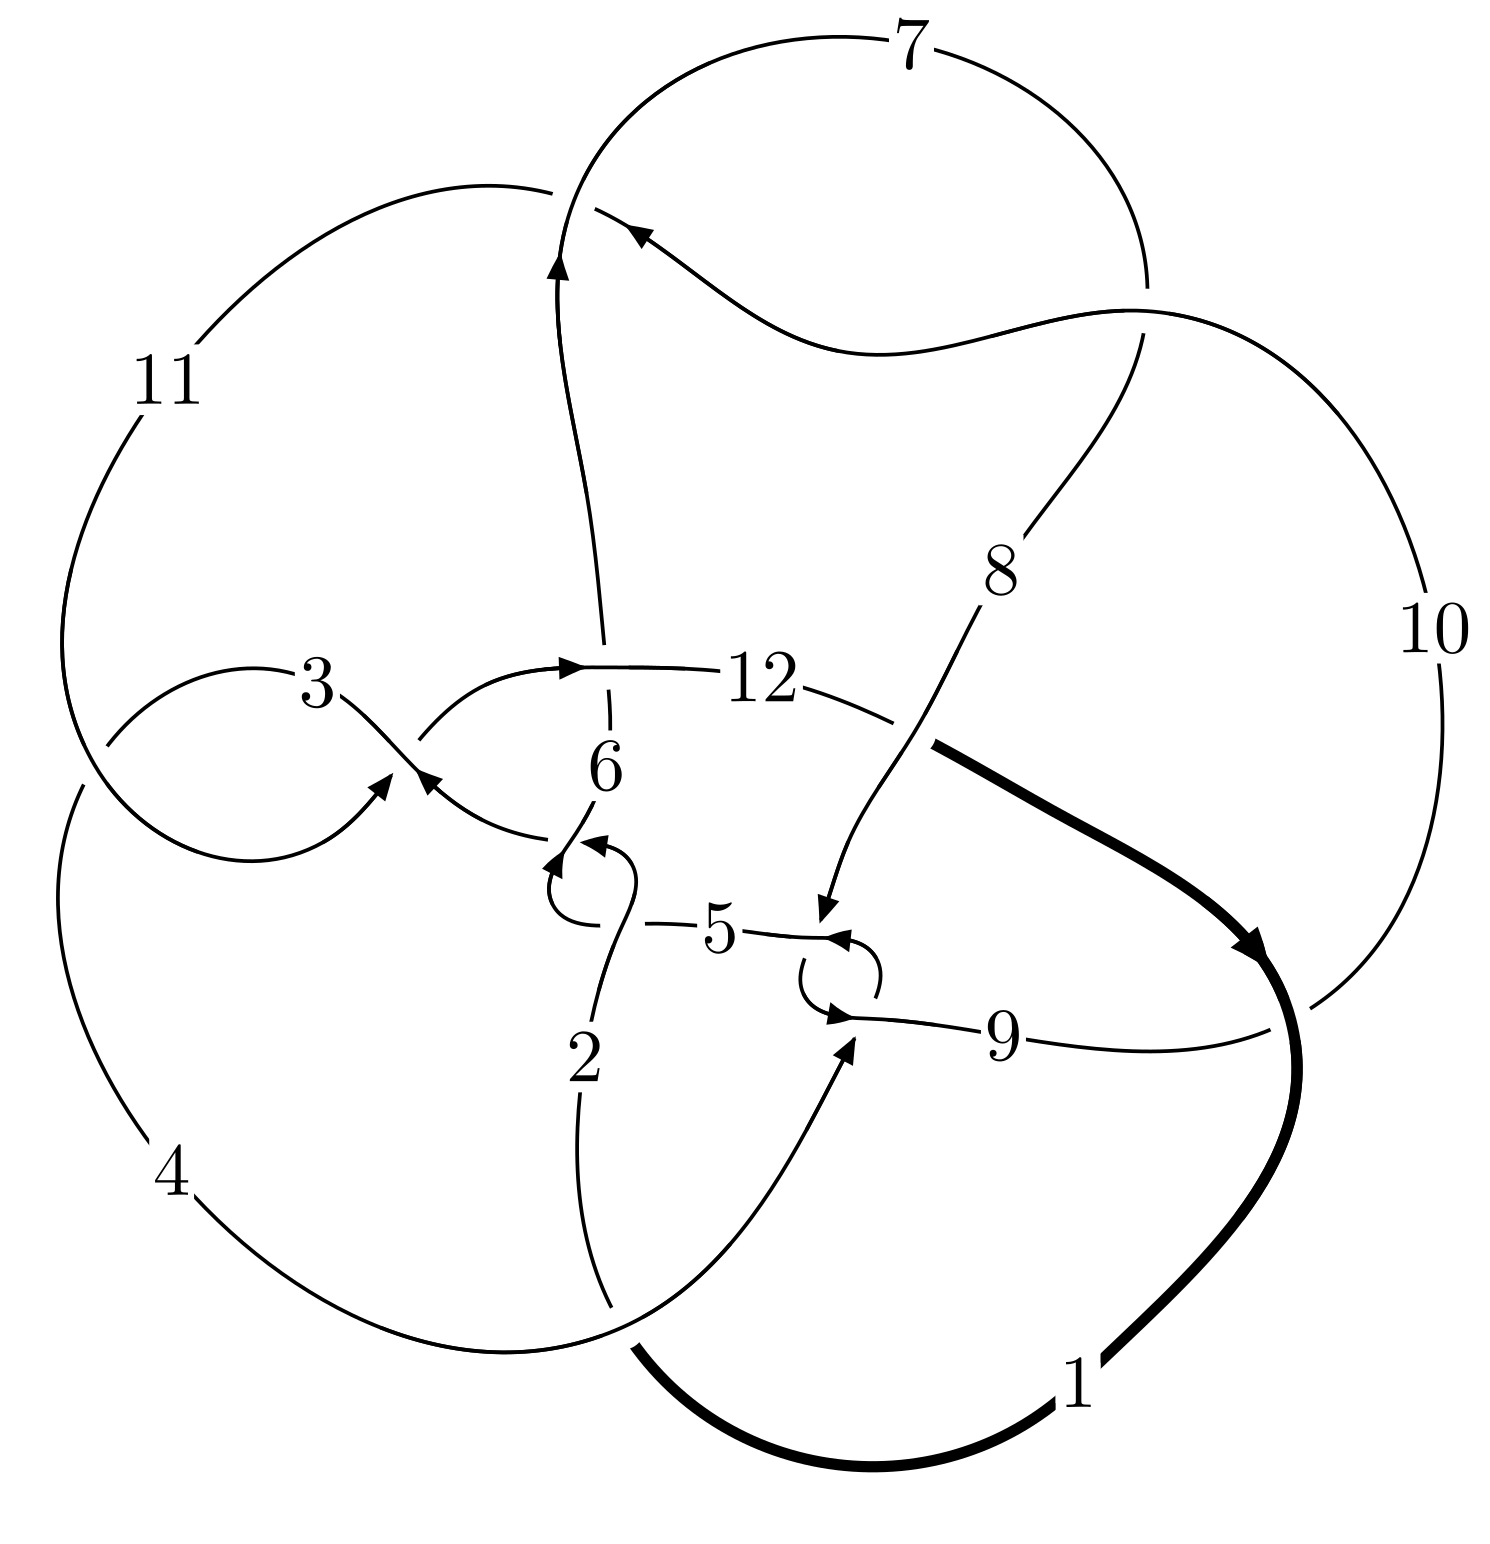
\includegraphics[width=112pt]{../../../GIT/diagram.site/Diagrams/png/1784_12a_0983.png}\\
\ \ \ A knot diagram\footnotemark}&
\allowdisplaybreaks
\textbf{Linearized knot diagam} \\
\cline{2-2}
 &
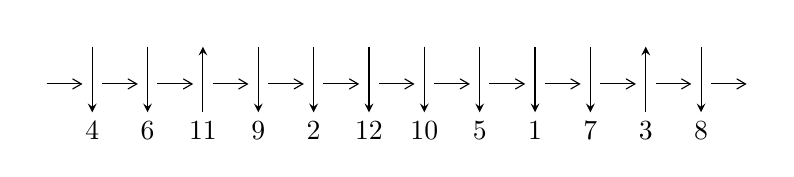
\begin{tikzpicture}[x=20pt, y=17pt]
	% nodes
	\node (C0) at (0, 0) {};
	\node (C1) at (1, 0) {};
	\node (C1U) at (1, +1) {};
	\node (C1D) at (1, -1) {4};

	\node (C2) at (2, 0) {};
	\node (C2U) at (2, +1) {};
	\node (C2D) at (2, -1) {6};

	\node (C3) at (3, 0) {};
	\node (C3U) at (3, +1) {};
	\node (C3D) at (3, -1) {11};

	\node (C4) at (4, 0) {};
	\node (C4U) at (4, +1) {};
	\node (C4D) at (4, -1) {9};

	\node (C5) at (5, 0) {};
	\node (C5U) at (5, +1) {};
	\node (C5D) at (5, -1) {2};

	\node (C6) at (6, 0) {};
	\node (C6U) at (6, +1) {};
	\node (C6D) at (6, -1) {12};

	\node (C7) at (7, 0) {};
	\node (C7U) at (7, +1) {};
	\node (C7D) at (7, -1) {10};

	\node (C8) at (8, 0) {};
	\node (C8U) at (8, +1) {};
	\node (C8D) at (8, -1) {5};

	\node (C9) at (9, 0) {};
	\node (C9U) at (9, +1) {};
	\node (C9D) at (9, -1) {1};

	\node (C10) at (10, 0) {};
	\node (C10U) at (10, +1) {};
	\node (C10D) at (10, -1) {7};

	\node (C11) at (11, 0) {};
	\node (C11U) at (11, +1) {};
	\node (C11D) at (11, -1) {3};

	\node (C12) at (12, 0) {};
	\node (C12U) at (12, +1) {};
	\node (C12D) at (12, -1) {8};
	\node (C13) at (13, 0) {};

	% arrows
	\draw[->,>={angle 60}]
	(C0) edge (C1) (C1) edge (C2) (C2) edge (C3) (C3) edge (C4) (C4) edge (C5) (C5) edge (C6) (C6) edge (C7) (C7) edge (C8) (C8) edge (C9) (C9) edge (C10) (C10) edge (C11) (C11) edge (C12) (C12) edge (C13) ;	\draw[->,>=stealth]
	(C1U) edge (C1D) (C2U) edge (C2D) (C3D) edge (C3U) (C4U) edge (C4D) (C5U) edge (C5D) (C6U) edge (C6D) (C7U) edge (C7D) (C8U) edge (C8D) (C9U) edge (C9D) (C10U) edge (C10D) (C11D) edge (C11U) (C12U) edge (C12D) ;
	\end{tikzpicture} \\
\hhline{~~} \\& 
\textbf{Solving Sequence} \\ \cline{2-2} 
 &
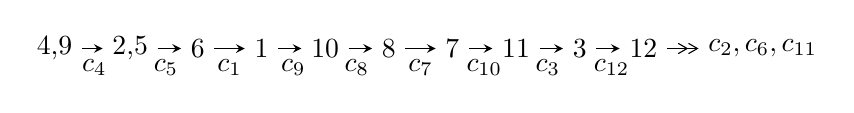
\begin{tikzpicture}[x=23pt, y=7pt]
	% node
	\node (A0) at (-1/8, 0) {4,9};
	\node (A1) at (17/16, 0) {2,5};
	\node (A2) at (17/8, 0) {6};
	\node (A3) at (25/8, 0) {1};
	\node (A4) at (33/8, 0) {10};
	\node (A5) at (41/8, 0) {8};
	\node (A6) at (49/8, 0) {7};
	\node (A7) at (57/8, 0) {11};
	\node (A8) at (65/8, 0) {3};
	\node (A9) at (73/8, 0) {12};
	\node (C1) at (1/2, -1) {$c_{4}$};
	\node (C2) at (13/8, -1) {$c_{5}$};
	\node (C3) at (21/8, -1) {$c_{1}$};
	\node (C4) at (29/8, -1) {$c_{9}$};
	\node (C5) at (37/8, -1) {$c_{8}$};
	\node (C6) at (45/8, -1) {$c_{7}$};
	\node (C7) at (53/8, -1) {$c_{10}$};
	\node (C8) at (61/8, -1) {$c_{3}$};
	\node (C9) at (69/8, -1) {$c_{12}$};
	\node (A10) at (11, 0) {$c_{2},c_{6},c_{11}$};

	% edge
	\draw[->,>=stealth]	
	(A0) edge (A1) (A1) edge (A2) (A2) edge (A3) (A3) edge (A4) (A4) edge (A5) (A5) edge (A6) (A6) edge (A7) (A7) edge (A8) (A8) edge (A9) ;
	\draw[->>,>={angle 60}]	
	(A9) edge (A10);
\end{tikzpicture} \\ 

\end{tabular} \\

\footnotetext{
The image of knot diagram is generated by the software ``\textbf{Draw programme}" developed by Andrew Bartholomew(\url{http://www.layer8.co.uk/maths/draw/index.htm\#Running-draw}), where we modified some parts for our purpose(\url{https://github.com/CATsTAILs/LinksPainter}).
}\phantom \\ \newline 
\centering \textbf{Ideals for irreducible components\footnotemark of $X_{\text{par}}$} 
 
\begin{align*}
I^u_{1}&=\langle 
9.08439\times10^{636} u^{154}-5.67777\times10^{637} u^{153}+\cdots+4.26910\times10^{637} b+4.02846\times10^{640},\\
\phantom{I^u_{1}}&\phantom{= \langle  }-1.96555\times10^{640} u^{154}+1.40998\times10^{641} u^{153}+\cdots+8.32047\times10^{640} a-1.35238\times10^{644},\\
\phantom{I^u_{1}}&\phantom{= \langle  }u^{155}-5 u^{154}+\cdots+5977 u-1949\rangle \\
I^u_{2}&=\langle 
-2.54107\times10^{23} u^{40}-6.68625\times10^{24} u^{39}+\cdots+4.56220\times10^{23} b-1.25601\times10^{25},\\
\phantom{I^u_{2}}&\phantom{= \langle  }-6.16269\times10^{22} u^{40}+3.14727\times10^{22} u^{39}+\cdots+6.42563\times10^{21} a+4.53567\times10^{22},\\
\phantom{I^u_{2}}&\phantom{= \langle  }u^{41}+12 u^{39}+\cdots+2 u+1\rangle \\
\\
\end{align*}
\raggedright * 2 irreducible components of $\dim_{\mathbb{C}}=0$, with total 196 representations.\\
\footnotetext{All coefficients of polynomials are rational numbers. But the coefficients are sometimes approximated in decimal forms when there is not enough margin.}
\newpage
\renewcommand{\arraystretch}{1}
\centering \section*{I. $I^u_{1}= \langle 9.08\times10^{636} u^{154}-5.68\times10^{637} u^{153}+\cdots+4.27\times10^{637} b+4.03\times10^{640},\;-1.97\times10^{640} u^{154}+1.41\times10^{641} u^{153}+\cdots+8.32\times10^{640} a-1.35\times10^{644},\;u^{155}-5 u^{154}+\cdots+5977 u-1949 \rangle$}
\flushleft \textbf{(i) Arc colorings}\\
\begin{tabular}{m{7pt} m{180pt} m{7pt} m{180pt} }
\flushright $a_{4}=$&$\begin{pmatrix}1\\0\end{pmatrix}$ \\
\flushright $a_{9}=$&$\begin{pmatrix}0\\u\end{pmatrix}$ \\
\flushright $a_{2}=$&$\begin{pmatrix}0.236230 u^{154}-1.69459 u^{153}+\cdots-5692.37 u+1625.37\\-0.212794 u^{154}+1.32997 u^{153}+\cdots+3632.61 u-943.634\end{pmatrix}$ \\
\flushright $a_{5}=$&$\begin{pmatrix}1\\u^2\end{pmatrix}$ \\
\flushright $a_{6}=$&$\begin{pmatrix}0.330331 u^{154}-1.99549 u^{153}+\cdots-3639.71 u+998.058\\-0.237444 u^{154}+1.28575 u^{153}+\cdots+2893.91 u-775.387\end{pmatrix}$ \\
\flushright $a_{1}=$&$\begin{pmatrix}0.0234361 u^{154}-0.364618 u^{153}+\cdots-2059.76 u+681.735\\-0.212794 u^{154}+1.32997 u^{153}+\cdots+3632.61 u-943.634\end{pmatrix}$ \\
\flushright $a_{10}=$&$\begin{pmatrix}0.189005 u^{154}-0.898469 u^{153}+\cdots+20.6553 u+13.2784\\0.120685 u^{154}-0.600088 u^{153}+\cdots+209.357 u-96.8051\end{pmatrix}$ \\
\flushright $a_{8}=$&$\begin{pmatrix}u\\u^3+u\end{pmatrix}$ \\
\flushright $a_{7}=$&$\begin{pmatrix}-0.0586751 u^{154}+0.174131 u^{153}+\cdots+1462.55 u-207.295\\0.109921 u^{154}-0.579575 u^{153}+\cdots+280.179 u-97.6014\end{pmatrix}$ \\
\flushright $a_{11}=$&$\begin{pmatrix}0.116953 u^{154}-0.407827 u^{153}+\cdots+2171.07 u-811.638\\0.166621 u^{154}-0.966567 u^{153}+\cdots+9.72642 u-32.9991\end{pmatrix}$ \\
\flushright $a_{3}=$&$\begin{pmatrix}0.168718 u^{154}-0.843287 u^{153}+\cdots-375.424 u-120.580\\0.275648 u^{154}-1.63163 u^{153}+\cdots-2328.86 u+541.989\end{pmatrix}$ \\
\flushright $a_{12}=$&$\begin{pmatrix}0.108998 u^{154}-0.940004 u^{153}+\cdots-4609.36 u+1398.34\\-0.194449 u^{154}+1.09618 u^{153}+\cdots+2131.83 u-514.656\end{pmatrix}$\\&\end{tabular}
\flushleft \textbf{(ii) Obstruction class $= -1$}\\~\\
\flushleft \textbf{(iii) Cusp Shapes $= 0.744791 u^{154}-3.25700 u^{153}+\cdots-2772.95 u-268.489$}\\~\\
\newpage\renewcommand{\arraystretch}{1}
\flushleft \textbf{(iv) u-Polynomials at the component}\newline \\
\begin{tabular}{m{50pt}|m{274pt}}
Crossings & \hspace{64pt}u-Polynomials at each crossing \\
\hline $$\begin{aligned}c_{1}\end{aligned}$$&$\begin{aligned}
&u^{155}-12 u^{154}+\cdots+27570093 u-1107493
\end{aligned}$\\
\hline $$\begin{aligned}c_{2},c_{5}\end{aligned}$$&$\begin{aligned}
&u^{155}+4 u^{154}+\cdots+3352225 u+213761
\end{aligned}$\\
\hline $$\begin{aligned}c_{3},c_{11}\end{aligned}$$&$\begin{aligned}
&u^{155}+46 u^{153}+\cdots+141090 u+6263
\end{aligned}$\\
\hline $$\begin{aligned}c_{4},c_{8}\end{aligned}$$&$\begin{aligned}
&u^{155}+5 u^{154}+\cdots+5977 u+1949
\end{aligned}$\\
\hline $$\begin{aligned}c_{6}\end{aligned}$$&$\begin{aligned}
&u^{155}+2 u^{154}+\cdots+2055676577 u+258968363
\end{aligned}$\\
\hline $$\begin{aligned}c_{7},c_{10}\end{aligned}$$&$\begin{aligned}
&u^{155}-8 u^{154}+\cdots-211061 u+8101
\end{aligned}$\\
\hline $$\begin{aligned}c_{9}\end{aligned}$$&$\begin{aligned}
&u^{155}+6 u^{154}+\cdots-6440321 u+1742611
\end{aligned}$\\
\hline $$\begin{aligned}c_{12}\end{aligned}$$&$\begin{aligned}
&u^{155}-2 u^{154}+\cdots-75394 u+5489
\end{aligned}$\\
\hline
\end{tabular}\\~\\
\newpage\renewcommand{\arraystretch}{1}
\flushleft \textbf{(v) Riley Polynomials at the component}\newline \\
\begin{tabular}{m{50pt}|m{274pt}}
Crossings & \hspace{64pt}Riley Polynomials at each crossing \\
\hline $$\begin{aligned}c_{1}\end{aligned}$$&$\begin{aligned}
&y^{155}+2 y^{154}+\cdots+738368560502371 y-1226540745049
\end{aligned}$\\
\hline $$\begin{aligned}c_{2},c_{5}\end{aligned}$$&$\begin{aligned}
&y^{155}-120 y^{154}+\cdots-8858040695633 y-45693765121
\end{aligned}$\\
\hline $$\begin{aligned}c_{3},c_{11}\end{aligned}$$&$\begin{aligned}
&y^{155}+92 y^{154}+\cdots+1224660764 y-39225169
\end{aligned}$\\
\hline $$\begin{aligned}c_{4},c_{8}\end{aligned}$$&$\begin{aligned}
&y^{155}+89 y^{154}+\cdots-114983845 y-3798601
\end{aligned}$\\
\hline $$\begin{aligned}c_{6}\end{aligned}$$&$\begin{aligned}
&y^{155}-34 y^{154}+\cdots+849943741672138741 y-67064613034899769
\end{aligned}$\\
\hline $$\begin{aligned}c_{7},c_{10}\end{aligned}$$&$\begin{aligned}
&y^{155}+110 y^{154}+\cdots-4992732509 y-65626201
\end{aligned}$\\
\hline $$\begin{aligned}c_{9}\end{aligned}$$&$\begin{aligned}
&y^{155}+52 y^{154}+\cdots-183271361272113 y-3036693097321
\end{aligned}$\\
\hline $$\begin{aligned}c_{12}\end{aligned}$$&$\begin{aligned}
&y^{155}+50 y^{154}+\cdots+2953027638 y-30129121
\end{aligned}$\\
\hline
\end{tabular}\\~\\
\newpage\flushleft \textbf{(vi) Complex Volumes and Cusp Shapes}
$$\begin{array}{c|c|c}  
\text{Solutions to }I^u_{1}& \I (\text{vol} + \sqrt{-1}CS) & \text{Cusp shape}\\
 \hline 
\begin{aligned}
u &= \phantom{-}0.632154 + 0.764495 I \\
a &= -1.18773 + 1.14589 I \\
b &= \phantom{-}0.656993 - 1.249390 I\end{aligned}
 & -1.52361 - 2.33822 I & \phantom{-0.000000 } 0 \\ \hline\begin{aligned}
u &= \phantom{-}0.632154 - 0.764495 I \\
a &= -1.18773 - 1.14589 I \\
b &= \phantom{-}0.656993 + 1.249390 I\end{aligned}
 & -1.52361 + 2.33822 I & \phantom{-0.000000 } 0 \\ \hline\begin{aligned}
u &= -0.332105 + 0.955418 I \\
a &= -0.88838 + 2.06421 I \\
b &= \phantom{-}0.428057 - 0.475116 I\end{aligned}
 & -5.98722 + 5.65625 I & \phantom{-0.000000 } 0 \\ \hline\begin{aligned}
u &= -0.332105 - 0.955418 I \\
a &= -0.88838 - 2.06421 I \\
b &= \phantom{-}0.428057 + 0.475116 I\end{aligned}
 & -5.98722 - 5.65625 I & \phantom{-0.000000 } 0 \\ \hline\begin{aligned}
u &= \phantom{-}0.320034 + 0.935213 I \\
a &= -1.44761 - 2.62074 I \\
b &= \phantom{-}1.58115 + 1.32042 I\end{aligned}
 & -2.69846 + 5.60305 I & \phantom{-0.000000 } 0 \\ \hline\begin{aligned}
u &= \phantom{-}0.320034 - 0.935213 I \\
a &= -1.44761 + 2.62074 I \\
b &= \phantom{-}1.58115 - 1.32042 I\end{aligned}
 & -2.69846 - 5.60305 I & \phantom{-0.000000 } 0 \\ \hline\begin{aligned}
u &= \phantom{-}0.165753 + 0.943595 I \\
a &= \phantom{-}0.586498 - 1.215400 I \\
b &= -1.55472 + 1.20228 I\end{aligned}
 & \phantom{-}2.07947 - 3.25255 I & \phantom{-0.000000 } 0 \\ \hline\begin{aligned}
u &= \phantom{-}0.165753 - 0.943595 I \\
a &= \phantom{-}0.586498 + 1.215400 I \\
b &= -1.55472 - 1.20228 I\end{aligned}
 & \phantom{-}2.07947 + 3.25255 I & \phantom{-0.000000 } 0 \\ \hline\begin{aligned}
u &= -0.336433 + 0.886864 I \\
a &= \phantom{-}0.49414 - 2.15802 I \\
b &= -0.475427 + 0.808420 I\end{aligned}
 & -2.73771 + 1.86517 I & \phantom{-0.000000 } 0 \\ \hline\begin{aligned}
u &= -0.336433 - 0.886864 I \\
a &= \phantom{-}0.49414 + 2.15802 I \\
b &= -0.475427 - 0.808420 I\end{aligned}
 & -2.73771 - 1.86517 I & \phantom{-0.000000 } 0\\
 \hline 
 \end{array}$$\newpage$$\begin{array}{c|c|c}  
\text{Solutions to }I^u_{1}& \I (\text{vol} + \sqrt{-1}CS) & \text{Cusp shape}\\
 \hline 
\begin{aligned}
u &= -0.947907 + 0.023227 I \\
a &= -0.254238 - 0.022444 I \\
b &= -0.412821 - 1.053730 I\end{aligned}
 & \phantom{-}1.60910 - 8.22629 I & \phantom{-0.000000 } 0 \\ \hline\begin{aligned}
u &= -0.947907 - 0.023227 I \\
a &= -0.254238 + 0.022444 I \\
b &= -0.412821 + 1.053730 I\end{aligned}
 & \phantom{-}1.60910 + 8.22629 I & \phantom{-0.000000 } 0 \\ \hline\begin{aligned}
u &= -0.388203 + 0.864670 I \\
a &= -0.31910 + 2.41589 I \\
b &= \phantom{-}0.63527 - 1.41490 I\end{aligned}
 & -6.60783 - 1.40063 I & \phantom{-0.000000 } 0 \\ \hline\begin{aligned}
u &= -0.388203 - 0.864670 I \\
a &= -0.31910 - 2.41589 I \\
b &= \phantom{-}0.63527 + 1.41490 I\end{aligned}
 & -6.60783 + 1.40063 I & \phantom{-0.000000 } 0 \\ \hline\begin{aligned}
u &= -0.308062 + 1.007630 I \\
a &= -0.28746 - 1.60359 I \\
b &= -1.00284 + 1.04042 I\end{aligned}
 & \phantom{-}1.21740 + 4.03535 I & \phantom{-0.000000 } 0 \\ \hline\begin{aligned}
u &= -0.308062 - 1.007630 I \\
a &= -0.28746 + 1.60359 I \\
b &= -1.00284 - 1.04042 I\end{aligned}
 & \phantom{-}1.21740 - 4.03535 I & \phantom{-0.000000 } 0 \\ \hline\begin{aligned}
u &= \phantom{-}1.060490 + 0.136755 I \\
a &= -0.395064 - 0.346887 I \\
b &= \phantom{-}0.941299 - 0.388243 I\end{aligned}
 & -6.64824 + 1.50984 I & \phantom{-0.000000 } 0 \\ \hline\begin{aligned}
u &= \phantom{-}1.060490 - 0.136755 I \\
a &= -0.395064 + 0.346887 I \\
b &= \phantom{-}0.941299 + 0.388243 I\end{aligned}
 & -6.64824 - 1.50984 I & \phantom{-0.000000 } 0 \\ \hline\begin{aligned}
u &= \phantom{-}0.464278 + 0.976770 I \\
a &= \phantom{-}0.30566 + 1.84213 I \\
b &= -0.728498 - 0.632407 I\end{aligned}
 & \phantom{-}0.02278 - 5.80615 I & \phantom{-0.000000 } 0 \\ \hline\begin{aligned}
u &= \phantom{-}0.464278 - 0.976770 I \\
a &= \phantom{-}0.30566 - 1.84213 I \\
b &= -0.728498 + 0.632407 I\end{aligned}
 & \phantom{-}0.02278 + 5.80615 I & \phantom{-0.000000 } 0\\
 \hline 
 \end{array}$$\newpage$$\begin{array}{c|c|c}  
\text{Solutions to }I^u_{1}& \I (\text{vol} + \sqrt{-1}CS) & \text{Cusp shape}\\
 \hline 
\begin{aligned}
u &= \phantom{-}0.440998 + 0.997274 I \\
a &= -0.68309 - 2.08178 I \\
b &= \phantom{-}1.040830 + 0.429714 I\end{aligned}
 & -3.47172 - 10.78400 I & \phantom{-0.000000 } 0 \\ \hline\begin{aligned}
u &= \phantom{-}0.440998 - 0.997274 I \\
a &= -0.68309 + 2.08178 I \\
b &= \phantom{-}1.040830 - 0.429714 I\end{aligned}
 & -3.47172 + 10.78400 I & \phantom{-0.000000 } 0 \\ \hline\begin{aligned}
u &= \phantom{-}0.630842 + 0.647374 I \\
a &= \phantom{-}1.07282 - 1.33346 I \\
b &= -0.292806 + 1.331150 I\end{aligned}
 & -1.80068 - 2.59274 I & \phantom{-0.000000 } 0 \\ \hline\begin{aligned}
u &= \phantom{-}0.630842 - 0.647374 I \\
a &= \phantom{-}1.07282 + 1.33346 I \\
b &= -0.292806 - 1.331150 I\end{aligned}
 & -1.80068 + 2.59274 I & \phantom{-0.000000 } 0 \\ \hline\begin{aligned}
u &= -0.902322 + 0.044640 I \\
a &= \phantom{-}0.418779 - 0.204155 I \\
b &= \phantom{-}0.275791 - 0.766068 I\end{aligned}
 & \phantom{-}3.96728 + 3.58960 I & \phantom{-0.000000 } 0 \\ \hline\begin{aligned}
u &= -0.902322 - 0.044640 I \\
a &= \phantom{-}0.418779 + 0.204155 I \\
b &= \phantom{-}0.275791 + 0.766068 I\end{aligned}
 & \phantom{-}3.96728 - 3.58960 I & \phantom{-0.000000 } 0 \\ \hline\begin{aligned}
u &= \phantom{-}0.155717 + 0.883135 I \\
a &= \phantom{-}1.05498 + 2.34477 I \\
b &= -0.271165 - 1.150490 I\end{aligned}
 & \phantom{-}1.90724 + 1.69368 I & \phantom{-0.000000 } 0 \\ \hline\begin{aligned}
u &= \phantom{-}0.155717 - 0.883135 I \\
a &= \phantom{-}1.05498 - 2.34477 I \\
b &= -0.271165 + 1.150490 I\end{aligned}
 & \phantom{-}1.90724 - 1.69368 I & \phantom{-0.000000 } 0 \\ \hline\begin{aligned}
u &= \phantom{-}0.407305 + 1.027460 I \\
a &= -0.59832 + 1.29563 I \\
b &= -1.23541 - 1.14072 I\end{aligned}
 & \phantom{-}4.63415 - 5.45186 I & \phantom{-0.000000 } 0 \\ \hline\begin{aligned}
u &= \phantom{-}0.407305 - 1.027460 I \\
a &= -0.59832 - 1.29563 I \\
b &= -1.23541 + 1.14072 I\end{aligned}
 & \phantom{-}4.63415 + 5.45186 I & \phantom{-0.000000 } 0\\
 \hline 
 \end{array}$$\newpage$$\begin{array}{c|c|c}  
\text{Solutions to }I^u_{1}& \I (\text{vol} + \sqrt{-1}CS) & \text{Cusp shape}\\
 \hline 
\begin{aligned}
u &= -0.655471 + 0.910338 I \\
a &= -0.331171 + 0.795825 I \\
b &= -0.369577 + 0.034401 I\end{aligned}
 & -3.65853 - 0.76921 I & \phantom{-0.000000 } 0 \\ \hline\begin{aligned}
u &= -0.655471 - 0.910338 I \\
a &= -0.331171 - 0.795825 I \\
b &= -0.369577 - 0.034401 I\end{aligned}
 & -3.65853 + 0.76921 I & \phantom{-0.000000 } 0 \\ \hline\begin{aligned}
u &= \phantom{-}0.219832 + 1.106170 I \\
a &= -0.968653 + 0.366699 I \\
b &= -0.622560 - 0.130561 I\end{aligned}
 & \phantom{-}3.44823 - 2.86027 I & \phantom{-0.000000 } 0 \\ \hline\begin{aligned}
u &= \phantom{-}0.219832 - 1.106170 I \\
a &= -0.968653 - 0.366699 I \\
b &= -0.622560 + 0.130561 I\end{aligned}
 & \phantom{-}3.44823 + 2.86027 I & \phantom{-0.000000 } 0 \\ \hline\begin{aligned}
u &= \phantom{-}0.665562 + 0.913944 I \\
a &= \phantom{-}1.15419 - 0.97993 I \\
b &= -0.28018 + 1.75138 I\end{aligned}
 & \phantom{-}3.33744 + 0.06742 I & \phantom{-0.000000 } 0 \\ \hline\begin{aligned}
u &= \phantom{-}0.665562 - 0.913944 I \\
a &= \phantom{-}1.15419 + 0.97993 I \\
b &= -0.28018 - 1.75138 I\end{aligned}
 & \phantom{-}3.33744 - 0.06742 I & \phantom{-0.000000 } 0 \\ \hline\begin{aligned}
u &= \phantom{-}0.853746 + 0.160759 I \\
a &= \phantom{-}0.386286 + 0.044218 I \\
b &= -0.445128 + 0.406798 I\end{aligned}
 & -1.042080 + 0.198583 I & \phantom{-0.000000 } 0 \\ \hline\begin{aligned}
u &= \phantom{-}0.853746 - 0.160759 I \\
a &= \phantom{-}0.386286 - 0.044218 I \\
b &= -0.445128 - 0.406798 I\end{aligned}
 & -1.042080 - 0.198583 I & \phantom{-0.000000 } 0 \\ \hline\begin{aligned}
u &= \phantom{-}1.104610 + 0.255028 I \\
a &= -0.507189 - 0.167972 I \\
b &= \phantom{-}0.936725 - 0.943509 I\end{aligned}
 & -3.47694 + 13.60270 I & \phantom{-0.000000 } 0 \\ \hline\begin{aligned}
u &= \phantom{-}1.104610 - 0.255028 I \\
a &= -0.507189 + 0.167972 I \\
b &= \phantom{-}0.936725 + 0.943509 I\end{aligned}
 & -3.47694 - 13.60270 I & \phantom{-0.000000 } 0\\
 \hline 
 \end{array}$$\newpage$$\begin{array}{c|c|c}  
\text{Solutions to }I^u_{1}& \I (\text{vol} + \sqrt{-1}CS) & \text{Cusp shape}\\
 \hline 
\begin{aligned}
u &= -0.145480 + 0.841695 I \\
a &= -0.42940 - 2.52384 I \\
b &= -0.503978 + 0.504682 I\end{aligned}
 & \phantom{-}0.06024 + 4.12457 I & \phantom{-0.000000 } 0 \\ \hline\begin{aligned}
u &= -0.145480 - 0.841695 I \\
a &= -0.42940 + 2.52384 I \\
b &= -0.503978 - 0.504682 I\end{aligned}
 & \phantom{-}0.06024 - 4.12457 I & \phantom{-0.000000 } 0 \\ \hline\begin{aligned}
u &= \phantom{-}0.210950 + 1.131710 I \\
a &= -0.07148 + 1.94014 I \\
b &= -0.64854 - 1.77286 I\end{aligned}
 & \phantom{-}5.15722 - 4.94782 I & \phantom{-0.000000 } 0 \\ \hline\begin{aligned}
u &= \phantom{-}0.210950 - 1.131710 I \\
a &= -0.07148 - 1.94014 I \\
b &= -0.64854 + 1.77286 I\end{aligned}
 & \phantom{-}5.15722 + 4.94782 I & \phantom{-0.000000 } 0 \\ \hline\begin{aligned}
u &= -0.217354 + 1.133410 I \\
a &= \phantom{-}0.433968 + 1.047940 I \\
b &= \phantom{-}0.497943 - 0.806490 I\end{aligned}
 & \phantom{-}3.40378 + 0.05786 I & \phantom{-0.000000 } 0 \\ \hline\begin{aligned}
u &= -0.217354 - 1.133410 I \\
a &= \phantom{-}0.433968 - 1.047940 I \\
b &= \phantom{-}0.497943 + 0.806490 I\end{aligned}
 & \phantom{-}3.40378 - 0.05786 I & \phantom{-0.000000 } 0 \\ \hline\begin{aligned}
u &= -0.379012 + 1.093380 I \\
a &= -0.971570 - 0.105723 I \\
b &= \phantom{-}0.135918 + 0.931279 I\end{aligned}
 & \phantom{-}4.11695 - 0.46339 I & \phantom{-0.000000 } 0 \\ \hline\begin{aligned}
u &= -0.379012 - 1.093380 I \\
a &= -0.971570 + 0.105723 I \\
b &= \phantom{-}0.135918 - 0.931279 I\end{aligned}
 & \phantom{-}4.11695 + 0.46339 I & \phantom{-0.000000 } 0 \\ \hline\begin{aligned}
u &= \phantom{-}0.174326 + 0.821465 I \\
a &= -2.40032 - 0.25977 I \\
b &= \phantom{-}2.98947 - 0.36087 I\end{aligned}
 & -3.37727 - 7.93787 I & \phantom{-0.000000 } 0 \\ \hline\begin{aligned}
u &= \phantom{-}0.174326 - 0.821465 I \\
a &= -2.40032 + 0.25977 I \\
b &= \phantom{-}2.98947 + 0.36087 I\end{aligned}
 & -3.37727 + 7.93787 I & \phantom{-0.000000 } 0\\
 \hline 
 \end{array}$$\newpage$$\begin{array}{c|c|c}  
\text{Solutions to }I^u_{1}& \I (\text{vol} + \sqrt{-1}CS) & \text{Cusp shape}\\
 \hline 
\begin{aligned}
u &= -0.279492 + 0.791159 I \\
a &= -0.052746 - 1.333800 I \\
b &= -0.697093 - 0.199773 I\end{aligned}
 & \phantom{-}0.21819 - 1.92183 I & \phantom{-0.000000 } 0 \\ \hline\begin{aligned}
u &= -0.279492 - 0.791159 I \\
a &= -0.052746 + 1.333800 I \\
b &= -0.697093 + 0.199773 I\end{aligned}
 & \phantom{-}0.21819 + 1.92183 I & \phantom{-0.000000 } 0 \\ \hline\begin{aligned}
u &= -0.667864 + 0.494882 I \\
a &= -0.199319 - 0.960026 I \\
b &= \phantom{-}0.803175 - 0.259614 I\end{aligned}
 & -4.77617 + 5.79352 I & \phantom{-0.000000 } 0 \\ \hline\begin{aligned}
u &= -0.667864 - 0.494882 I \\
a &= -0.199319 + 0.960026 I \\
b &= \phantom{-}0.803175 + 0.259614 I\end{aligned}
 & -4.77617 - 5.79352 I & \phantom{-0.000000 } 0 \\ \hline\begin{aligned}
u &= \phantom{-}0.593305 + 1.007890 I \\
a &= -0.88677 + 1.59849 I \\
b &= -0.32755 - 1.80236 I\end{aligned}
 & \phantom{-}3.69654 - 5.06498 I & \phantom{-0.000000 } 0 \\ \hline\begin{aligned}
u &= \phantom{-}0.593305 - 1.007890 I \\
a &= -0.88677 - 1.59849 I \\
b &= -0.32755 + 1.80236 I\end{aligned}
 & \phantom{-}3.69654 + 5.06498 I & \phantom{-0.000000 } 0 \\ \hline\begin{aligned}
u &= \phantom{-}0.064119 + 0.824612 I \\
a &= \phantom{-}1.13744 + 2.27781 I \\
b &= -0.005073 - 0.691467 I\end{aligned}
 & \phantom{-}2.03577 + 1.68642 I & \phantom{-0.000000 } 0 \\ \hline\begin{aligned}
u &= \phantom{-}0.064119 - 0.824612 I \\
a &= \phantom{-}1.13744 - 2.27781 I \\
b &= -0.005073 + 0.691467 I\end{aligned}
 & \phantom{-}2.03577 - 1.68642 I & \phantom{-0.000000 } 0 \\ \hline\begin{aligned}
u &= \phantom{-}0.782761 + 0.261434 I \\
a &= -0.298402 + 0.700222 I \\
b &= -0.517502 - 0.534657 I\end{aligned}
 & -3.70924 - 1.83954 I & \phantom{-0.000000 } 0 \\ \hline\begin{aligned}
u &= \phantom{-}0.782761 - 0.261434 I \\
a &= -0.298402 - 0.700222 I \\
b &= -0.517502 + 0.534657 I\end{aligned}
 & -3.70924 + 1.83954 I & \phantom{-0.000000 } 0\\
 \hline 
 \end{array}$$\newpage$$\begin{array}{c|c|c}  
\text{Solutions to }I^u_{1}& \I (\text{vol} + \sqrt{-1}CS) & \text{Cusp shape}\\
 \hline 
\begin{aligned}
u &= \phantom{-}0.398255 + 1.107460 I \\
a &= \phantom{-}0.297301 + 0.172591 I \\
b &= -0.837825 - 0.163613 I\end{aligned}
 & -1.32317 - 2.47298 I & \phantom{-0.000000 } 0 \\ \hline\begin{aligned}
u &= \phantom{-}0.398255 - 1.107460 I \\
a &= \phantom{-}0.297301 - 0.172591 I \\
b &= -0.837825 + 0.163613 I\end{aligned}
 & -1.32317 + 2.47298 I & \phantom{-0.000000 } 0 \\ \hline\begin{aligned}
u &= \phantom{-}0.548751 + 1.041890 I \\
a &= -0.533329 - 1.037770 I \\
b &= \phantom{-}0.316666 + 0.111508 I\end{aligned}
 & -3.73870 - 1.26130 I & \phantom{-0.000000 } 0 \\ \hline\begin{aligned}
u &= \phantom{-}0.548751 - 1.041890 I \\
a &= -0.533329 + 1.037770 I \\
b &= \phantom{-}0.316666 - 0.111508 I\end{aligned}
 & -3.73870 + 1.26130 I & \phantom{-0.000000 } 0 \\ \hline\begin{aligned}
u &= -0.328741 + 1.130950 I \\
a &= \phantom{-}0.890426 - 0.905705 I \\
b &= -1.72705 + 0.48694 I\end{aligned}
 & \phantom{-}1.25479 + 6.54912 I & \phantom{-0.000000 } 0 \\ \hline\begin{aligned}
u &= -0.328741 - 1.130950 I \\
a &= \phantom{-}0.890426 + 0.905705 I \\
b &= -1.72705 - 0.48694 I\end{aligned}
 & \phantom{-}1.25479 - 6.54912 I & \phantom{-0.000000 } 0 \\ \hline\begin{aligned}
u &= -0.315353 + 0.748878 I \\
a &= -1.54231 - 0.64173 I \\
b &= \phantom{-}1.82527 + 0.83218 I\end{aligned}
 & -7.05962 + 4.60091 I & \phantom{-0.000000 } 0 \\ \hline\begin{aligned}
u &= -0.315353 - 0.748878 I \\
a &= -1.54231 + 0.64173 I \\
b &= \phantom{-}1.82527 - 0.83218 I\end{aligned}
 & -7.05962 - 4.60091 I & \phantom{-0.000000 } 0 \\ \hline\begin{aligned}
u &= \phantom{-}1.164350 + 0.245956 I \\
a &= \phantom{-}0.447906 + 0.184566 I \\
b &= -0.781624 + 0.785430 I\end{aligned}
 & \phantom{-}0.20952 + 6.87027 I & \phantom{-0.000000 } 0 \\ \hline\begin{aligned}
u &= \phantom{-}1.164350 - 0.245956 I \\
a &= \phantom{-}0.447906 - 0.184566 I \\
b &= -0.781624 - 0.785430 I\end{aligned}
 & \phantom{-}0.20952 - 6.87027 I & \phantom{-0.000000 } 0\\
 \hline 
 \end{array}$$\newpage$$\begin{array}{c|c|c}  
\text{Solutions to }I^u_{1}& \I (\text{vol} + \sqrt{-1}CS) & \text{Cusp shape}\\
 \hline 
\begin{aligned}
u &= \phantom{-}0.442189 + 1.110960 I \\
a &= \phantom{-}0.98886 - 1.05193 I \\
b &= \phantom{-}0.649432 + 1.200950 I\end{aligned}
 & \phantom{-}4.17031 - 1.59616 I & \phantom{-0.000000 } 0 \\ \hline\begin{aligned}
u &= \phantom{-}0.442189 - 1.110960 I \\
a &= \phantom{-}0.98886 + 1.05193 I \\
b &= \phantom{-}0.649432 - 1.200950 I\end{aligned}
 & \phantom{-}4.17031 + 1.59616 I & \phantom{-0.000000 } 0 \\ \hline\begin{aligned}
u &= -0.309217 + 0.735277 I \\
a &= \phantom{-}0.341028 + 0.397452 I \\
b &= -1.335460 - 0.412926 I\end{aligned}
 & -3.24796 + 1.11316 I & \phantom{-0.000000 } 0 \\ \hline\begin{aligned}
u &= -0.309217 - 0.735277 I \\
a &= \phantom{-}0.341028 - 0.397452 I \\
b &= -1.335460 + 0.412926 I\end{aligned}
 & -3.24796 - 1.11316 I & \phantom{-0.000000 } 0 \\ \hline\begin{aligned}
u &= -0.768328 + 0.188401 I \\
a &= \phantom{-}0.275738 - 0.566334 I \\
b &= -0.871620 - 0.946838 I\end{aligned}
 & \phantom{-}0.32900 - 2.38674 I & \phantom{-0.000000 } 0 \\ \hline\begin{aligned}
u &= -0.768328 - 0.188401 I \\
a &= \phantom{-}0.275738 + 0.566334 I \\
b &= -0.871620 + 0.946838 I\end{aligned}
 & \phantom{-}0.32900 + 2.38674 I & \phantom{-0.000000 } 0 \\ \hline\begin{aligned}
u &= -0.354167 + 1.158710 I \\
a &= \phantom{-}1.059200 + 0.778046 I \\
b &= \phantom{-}0.067922 - 1.155330 I\end{aligned}
 & \phantom{-}4.32208 + 1.17221 I & \phantom{-0.000000 } 0 \\ \hline\begin{aligned}
u &= -0.354167 - 1.158710 I \\
a &= \phantom{-}1.059200 - 0.778046 I \\
b &= \phantom{-}0.067922 + 1.155330 I\end{aligned}
 & \phantom{-}4.32208 - 1.17221 I & \phantom{-0.000000 } 0 \\ \hline\begin{aligned}
u &= -1.175620 + 0.322537 I \\
a &= -0.465550 - 0.054229 I \\
b &= \phantom{-}0.779649 + 0.753123 I\end{aligned}
 & -8.26316 - 7.06323 I & \phantom{-0.000000 } 0 \\ \hline\begin{aligned}
u &= -1.175620 - 0.322537 I \\
a &= -0.465550 + 0.054229 I \\
b &= \phantom{-}0.779649 - 0.753123 I\end{aligned}
 & -8.26316 + 7.06323 I & \phantom{-0.000000 } 0\\
 \hline 
 \end{array}$$\newpage$$\begin{array}{c|c|c}  
\text{Solutions to }I^u_{1}& \I (\text{vol} + \sqrt{-1}CS) & \text{Cusp shape}\\
 \hline 
\begin{aligned}
u &= \phantom{-}0.622512 + 0.453662 I \\
a &= \phantom{-}0.0266475 - 0.0692873 I \\
b &= -1.227340 + 0.239113 I\end{aligned}
 & -1.47244 + 1.58934 I & \phantom{-0.000000 } 0 \\ \hline\begin{aligned}
u &= \phantom{-}0.622512 - 0.453662 I \\
a &= \phantom{-}0.0266475 + 0.0692873 I \\
b &= -1.227340 - 0.239113 I\end{aligned}
 & -1.47244 - 1.58934 I & \phantom{-0.000000 } 0 \\ \hline\begin{aligned}
u &= -1.142530 + 0.505732 I \\
a &= \phantom{-}0.523359 + 0.032096 I \\
b &= -0.543675 - 0.766771 I\end{aligned}
 & -2.87889 - 1.93304 I & \phantom{-0.000000 } 0 \\ \hline\begin{aligned}
u &= -1.142530 - 0.505732 I \\
a &= \phantom{-}0.523359 - 0.032096 I \\
b &= -0.543675 + 0.766771 I\end{aligned}
 & -2.87889 + 1.93304 I & \phantom{-0.000000 } 0 \\ \hline\begin{aligned}
u &= \phantom{-}0.043575 + 1.249060 I \\
a &= -0.435578 - 0.988161 I \\
b &= \phantom{-}1.08789 + 1.05730 I\end{aligned}
 & \phantom{-}7.75572 + 1.57249 I & \phantom{-0.000000 } 0 \\ \hline\begin{aligned}
u &= \phantom{-}0.043575 - 1.249060 I \\
a &= -0.435578 + 0.988161 I \\
b &= \phantom{-}1.08789 - 1.05730 I\end{aligned}
 & \phantom{-}7.75572 - 1.57249 I & \phantom{-0.000000 } 0 \\ \hline\begin{aligned}
u &= \phantom{-}0.289936 + 1.219130 I \\
a &= \phantom{-}0.99461 - 1.01004 I \\
b &= \phantom{-}0.393519 + 0.626484 I\end{aligned}
 & \phantom{-}3.20983 - 4.81140 I & \phantom{-0.000000 } 0 \\ \hline\begin{aligned}
u &= \phantom{-}0.289936 - 1.219130 I \\
a &= \phantom{-}0.99461 + 1.01004 I \\
b &= \phantom{-}0.393519 - 0.626484 I\end{aligned}
 & \phantom{-}3.20983 + 4.81140 I & \phantom{-0.000000 } 0 \\ \hline\begin{aligned}
u &= -0.506429 + 1.146790 I \\
a &= -0.35114 + 2.11186 I \\
b &= \phantom{-}1.70814 - 1.58659 I\end{aligned}
 & \phantom{-}3.20415 + 8.25375 I & \phantom{-0.000000 } 0 \\ \hline\begin{aligned}
u &= -0.506429 - 1.146790 I \\
a &= -0.35114 - 2.11186 I \\
b &= \phantom{-}1.70814 + 1.58659 I\end{aligned}
 & \phantom{-}3.20415 - 8.25375 I & \phantom{-0.000000 } 0\\
 \hline 
 \end{array}$$\newpage$$\begin{array}{c|c|c}  
\text{Solutions to }I^u_{1}& \I (\text{vol} + \sqrt{-1}CS) & \text{Cusp shape}\\
 \hline 
\begin{aligned}
u &= -0.698177 + 0.220233 I \\
a &= -0.419829 + 1.074660 I \\
b &= \phantom{-}1.31140 + 0.67801 I\end{aligned}
 & \phantom{-}0.51455 - 3.66015 I & \phantom{-0.000000 } 0 \\ \hline\begin{aligned}
u &= -0.698177 - 0.220233 I \\
a &= -0.419829 - 1.074660 I \\
b &= \phantom{-}1.31140 - 0.67801 I\end{aligned}
 & \phantom{-}0.51455 + 3.66015 I & \phantom{-0.000000 } 0 \\ \hline\begin{aligned}
u &= -0.278021 + 1.247040 I \\
a &= -0.98662 + 1.95880 I \\
b &= \phantom{-}1.43804 - 1.92991 I\end{aligned}
 & \phantom{-}0.15735 + 8.43497 I & \phantom{-0.000000 } 0 \\ \hline\begin{aligned}
u &= -0.278021 - 1.247040 I \\
a &= -0.98662 - 1.95880 I \\
b &= \phantom{-}1.43804 + 1.92991 I\end{aligned}
 & \phantom{-}0.15735 - 8.43497 I & \phantom{-0.000000 } 0 \\ \hline\begin{aligned}
u &= -0.514734 + 1.170450 I \\
a &= -0.08794 - 1.94033 I \\
b &= -1.30080 + 1.60796 I\end{aligned}
 & \phantom{-}3.21663 + 7.16288 I & \phantom{-0.000000 } 0 \\ \hline\begin{aligned}
u &= -0.514734 - 1.170450 I \\
a &= -0.08794 + 1.94033 I \\
b &= -1.30080 - 1.60796 I\end{aligned}
 & \phantom{-}3.21663 - 7.16288 I & \phantom{-0.000000 } 0 \\ \hline\begin{aligned}
u &= \phantom{-}0.412246 + 1.221430 I \\
a &= \phantom{-}0.438540 - 0.919186 I \\
b &= \phantom{-}0.574472 + 0.762339 I\end{aligned}
 & \phantom{-}2.95233 - 3.87355 I & \phantom{-0.000000 } 0 \\ \hline\begin{aligned}
u &= \phantom{-}0.412246 - 1.221430 I \\
a &= \phantom{-}0.438540 + 0.919186 I \\
b &= \phantom{-}0.574472 - 0.762339 I\end{aligned}
 & \phantom{-}2.95233 + 3.87355 I & \phantom{-0.000000 } 0 \\ \hline\begin{aligned}
u &= \phantom{-}0.426286 + 1.219960 I \\
a &= -0.66481 - 1.78704 I \\
b &= \phantom{-}1.43638 + 1.38473 I\end{aligned}
 & -2.26989 - 7.19888 I & \phantom{-0.000000 } 0 \\ \hline\begin{aligned}
u &= \phantom{-}0.426286 - 1.219960 I \\
a &= -0.66481 + 1.78704 I \\
b &= \phantom{-}1.43638 - 1.38473 I\end{aligned}
 & -2.26989 + 7.19888 I & \phantom{-0.000000 } 0\\
 \hline 
 \end{array}$$\newpage$$\begin{array}{c|c|c}  
\text{Solutions to }I^u_{1}& \I (\text{vol} + \sqrt{-1}CS) & \text{Cusp shape}\\
 \hline 
\begin{aligned}
u &= -0.243161 + 0.664104 I \\
a &= \phantom{-}0.523133 - 0.354393 I \\
b &= \phantom{-}1.323260 + 0.243075 I\end{aligned}
 & -6.99155 - 2.85050 I & \phantom{-0.000000 } 0 \\ \hline\begin{aligned}
u &= -0.243161 - 0.664104 I \\
a &= \phantom{-}0.523133 + 0.354393 I \\
b &= \phantom{-}1.323260 - 0.243075 I\end{aligned}
 & -6.99155 + 2.85050 I & \phantom{-0.000000 } 0 \\ \hline\begin{aligned}
u &= \phantom{-}0.515308 + 1.203210 I \\
a &= -0.09123 + 1.52106 I \\
b &= -0.76313 - 1.26992 I\end{aligned}
 & \phantom{-}2.13886 - 5.12719 I & \phantom{-0.000000 } 0 \\ \hline\begin{aligned}
u &= \phantom{-}0.515308 - 1.203210 I \\
a &= -0.09123 - 1.52106 I \\
b &= -0.76313 + 1.26992 I\end{aligned}
 & \phantom{-}2.13886 + 5.12719 I & \phantom{-0.000000 } 0 \\ \hline\begin{aligned}
u &= -0.335508 + 0.597688 I \\
a &= \phantom{-}0.865218 + 1.033820 I \\
b &= \phantom{-}0.331892 + 0.033728 I\end{aligned}
 & \phantom{-}2.75467 + 1.57364 I & \phantom{-0.000000 } 0 \\ \hline\begin{aligned}
u &= -0.335508 - 0.597688 I \\
a &= \phantom{-}0.865218 - 1.033820 I \\
b &= \phantom{-}0.331892 - 0.033728 I\end{aligned}
 & \phantom{-}2.75467 - 1.57364 I & \phantom{-0.000000 } 0 \\ \hline\begin{aligned}
u &= \phantom{-}0.664010 + 0.151032 I \\
a &= -0.178023 + 0.640797 I \\
b &= \phantom{-}1.199990 + 0.348926 I\end{aligned}
 & -6.07050 - 3.24646 I & \phantom{-0.000000 } 0 \\ \hline\begin{aligned}
u &= \phantom{-}0.664010 - 0.151032 I \\
a &= -0.178023 - 0.640797 I \\
b &= \phantom{-}1.199990 - 0.348926 I\end{aligned}
 & -6.07050 + 3.24646 I & \phantom{-0.000000 } 0 \\ \hline\begin{aligned}
u &= \phantom{-}0.037284 + 1.334640 I \\
a &= -0.465607 - 0.486813 I \\
b &= -0.147167 + 0.263317 I\end{aligned}
 & -0.95180 - 2.88072 I & \phantom{-0.000000 } 0 \\ \hline\begin{aligned}
u &= \phantom{-}0.037284 - 1.334640 I \\
a &= -0.465607 + 0.486813 I \\
b &= -0.147167 - 0.263317 I\end{aligned}
 & -0.95180 + 2.88072 I & \phantom{-0.000000 } 0\\
 \hline 
 \end{array}$$\newpage$$\begin{array}{c|c|c}  
\text{Solutions to }I^u_{1}& \I (\text{vol} + \sqrt{-1}CS) & \text{Cusp shape}\\
 \hline 
\begin{aligned}
u &= -0.467731 + 1.262170 I \\
a &= \phantom{-}0.308949 + 1.136310 I \\
b &= \phantom{-}0.882237 - 0.995385 I\end{aligned}
 & \phantom{-}7.89563 + 8.39932 I & \phantom{-0.000000 } 0 \\ \hline\begin{aligned}
u &= -0.467731 - 1.262170 I \\
a &= \phantom{-}0.308949 - 1.136310 I \\
b &= \phantom{-}0.882237 + 0.995385 I\end{aligned}
 & \phantom{-}7.89563 - 8.39932 I & \phantom{-0.000000 } 0 \\ \hline\begin{aligned}
u &= \phantom{-}0.454528 + 0.468295 I \\
a &= \phantom{-}0.466447 - 0.293460 I \\
b &= \phantom{-}1.55447 - 0.20447 I\end{aligned}
 & -5.00548 + 6.98572 I & -12.81869 + 0. I\phantom{ +0.000000I} \\ \hline\begin{aligned}
u &= \phantom{-}0.454528 - 0.468295 I \\
a &= \phantom{-}0.466447 + 0.293460 I \\
b &= \phantom{-}1.55447 + 0.20447 I\end{aligned}
 & -5.00548 - 6.98572 I & -12.81869 + 0. I\phantom{ +0.000000I} \\ \hline\begin{aligned}
u &= -0.495947 + 1.269820 I \\
a &= -0.48329 - 1.41042 I \\
b &= -0.80391 + 1.22983 I\end{aligned}
 & \phantom{-}5.4234 + 13.3296 I & \phantom{-0.000000 } 0 \\ \hline\begin{aligned}
u &= -0.495947 - 1.269820 I \\
a &= -0.48329 + 1.41042 I \\
b &= -0.80391 - 1.22983 I\end{aligned}
 & \phantom{-}5.4234 - 13.3296 I & \phantom{-0.000000 } 0 \\ \hline\begin{aligned}
u &= -0.480158 + 1.308130 I \\
a &= -0.238432 - 0.965969 I \\
b &= -0.344087 + 1.131670 I\end{aligned}
 & \phantom{-}7.82001 + 1.55003 I & \phantom{-0.000000 } 0 \\ \hline\begin{aligned}
u &= -0.480158 - 1.308130 I \\
a &= -0.238432 + 0.965969 I \\
b &= -0.344087 - 1.131670 I\end{aligned}
 & \phantom{-}7.82001 - 1.55003 I & \phantom{-0.000000 } 0 \\ \hline\begin{aligned}
u &= -0.435470 + 1.327730 I \\
a &= \phantom{-}0.579421 + 1.018310 I \\
b &= \phantom{-}0.060548 - 1.164660 I\end{aligned}
 & \phantom{-}5.86004 - 3.19383 I & \phantom{-0.000000 } 0 \\ \hline\begin{aligned}
u &= -0.435470 - 1.327730 I \\
a &= \phantom{-}0.579421 - 1.018310 I \\
b &= \phantom{-}0.060548 + 1.164660 I\end{aligned}
 & \phantom{-}5.86004 + 3.19383 I & \phantom{-0.000000 } 0\\
 \hline 
 \end{array}$$\newpage$$\begin{array}{c|c|c}  
\text{Solutions to }I^u_{1}& \I (\text{vol} + \sqrt{-1}CS) & \text{Cusp shape}\\
 \hline 
\begin{aligned}
u &= \phantom{-}0.576786 + 0.166456 I \\
a &= \phantom{-}0.432897 - 0.994142 I \\
b &= -0.098592 - 0.980102 I\end{aligned}
 & \phantom{-}1.55147 - 2.37026 I & -8.00000 + 3.44366 I \\ \hline\begin{aligned}
u &= \phantom{-}0.576786 - 0.166456 I \\
a &= \phantom{-}0.432897 + 0.994142 I \\
b &= -0.098592 + 0.980102 I\end{aligned}
 & \phantom{-}1.55147 + 2.37026 I & -8.00000 - 3.44366 I \\ \hline\begin{aligned}
u &= -1.289590 + 0.546873 I \\
a &= -0.497506 - 0.030286 I \\
b &= \phantom{-}0.450415 + 0.496218 I\end{aligned}
 & -6.53330 + 4.97775 I & \phantom{-0.000000 } 0 \\ \hline\begin{aligned}
u &= -1.289590 - 0.546873 I \\
a &= -0.497506 + 0.030286 I \\
b &= \phantom{-}0.450415 - 0.496218 I\end{aligned}
 & -6.53330 - 4.97775 I & \phantom{-0.000000 } 0 \\ \hline\begin{aligned}
u &= \phantom{-}0.441209 + 1.329830 I \\
a &= -0.33967 + 1.44345 I \\
b &= -0.524598 - 1.002640 I\end{aligned}
 & \phantom{-}1.17347 - 6.29813 I & \phantom{-0.000000 } 0 \\ \hline\begin{aligned}
u &= \phantom{-}0.441209 - 1.329830 I \\
a &= -0.33967 - 1.44345 I \\
b &= -0.524598 + 1.002640 I\end{aligned}
 & \phantom{-}1.17347 + 6.29813 I & \phantom{-0.000000 } 0 \\ \hline\begin{aligned}
u &= -0.679370 + 1.231340 I \\
a &= -0.170929 - 1.330400 I \\
b &= -0.80144 + 1.29353 I\end{aligned}
 & -0.38329 + 8.43734 I & \phantom{-0.000000 } 0 \\ \hline\begin{aligned}
u &= -0.679370 - 1.231340 I \\
a &= -0.170929 + 1.330400 I \\
b &= -0.80144 - 1.29353 I\end{aligned}
 & -0.38329 - 8.43734 I & \phantom{-0.000000 } 0 \\ \hline\begin{aligned}
u &= \phantom{-}1.32290 + 0.51746 I \\
a &= -0.190207 + 0.430256 I \\
b &= \phantom{-}0.118271 - 0.626537 I\end{aligned}
 & -4.49216 - 1.70932 I & \phantom{-0.000000 } 0 \\ \hline\begin{aligned}
u &= \phantom{-}1.32290 - 0.51746 I \\
a &= -0.190207 - 0.430256 I \\
b &= \phantom{-}0.118271 + 0.626537 I\end{aligned}
 & -4.49216 + 1.70932 I & \phantom{-0.000000 } 0\\
 \hline 
 \end{array}$$\newpage$$\begin{array}{c|c|c}  
\text{Solutions to }I^u_{1}& \I (\text{vol} + \sqrt{-1}CS) & \text{Cusp shape}\\
 \hline 
\begin{aligned}
u &= \phantom{-}0.375658 + 0.440001 I \\
a &= \phantom{-}0.64923 + 1.87094 I \\
b &= -0.314859 + 0.570720 I\end{aligned}
 & \phantom{-}2.96714 + 1.99436 I & -4.69488 - 1.20406 I \\ \hline\begin{aligned}
u &= \phantom{-}0.375658 - 0.440001 I \\
a &= \phantom{-}0.64923 - 1.87094 I \\
b &= -0.314859 - 0.570720 I\end{aligned}
 & \phantom{-}2.96714 - 1.99436 I & -4.69488 + 1.20406 I \\ \hline\begin{aligned}
u &= \phantom{-}0.62937 + 1.27748 I \\
a &= -0.00293 - 1.67751 I \\
b &= \phantom{-}1.18421 + 1.53311 I\end{aligned}
 & -0.2572 - 19.7583 I & \phantom{-0.000000 } 0 \\ \hline\begin{aligned}
u &= \phantom{-}0.62937 - 1.27748 I \\
a &= -0.00293 + 1.67751 I \\
b &= \phantom{-}1.18421 - 1.53311 I\end{aligned}
 & -0.2572 + 19.7583 I & \phantom{-0.000000 } 0 \\ \hline\begin{aligned}
u &= \phantom{-}0.54728 + 1.31582 I \\
a &= -0.47652 - 1.33782 I \\
b &= \phantom{-}1.32944 + 1.11610 I\end{aligned}
 & -2.91923 - 7.22256 I & \phantom{-0.000000 } 0 \\ \hline\begin{aligned}
u &= \phantom{-}0.54728 - 1.31582 I \\
a &= -0.47652 + 1.33782 I \\
b &= \phantom{-}1.32944 - 1.11610 I\end{aligned}
 & -2.91923 + 7.22256 I & \phantom{-0.000000 } 0 \\ \hline\begin{aligned}
u &= \phantom{-}0.573688\phantom{ +0.000000I} \\
a &= \phantom{-}0.646215\phantom{ +0.000000I} \\
b &= \phantom{-}0.0411893\phantom{ +0.000000I}\end{aligned}
 & -0.844639\phantom{ +0.000000I} & -10.8360\phantom{ +0.000000I} \\ \hline\begin{aligned}
u &= -0.65115 + 1.27711 I \\
a &= \phantom{-}0.00968 + 1.52279 I \\
b &= \phantom{-}0.96355 - 1.30179 I\end{aligned}
 & -5.1619 + 13.4798 I & \phantom{-0.000000 } 0 \\ \hline\begin{aligned}
u &= -0.65115 - 1.27711 I \\
a &= \phantom{-}0.00968 - 1.52279 I \\
b &= \phantom{-}0.96355 + 1.30179 I\end{aligned}
 & -5.1619 - 13.4798 I & \phantom{-0.000000 } 0 \\ \hline\begin{aligned}
u &= \phantom{-}0.63931 + 1.29926 I \\
a &= \phantom{-}0.03131 + 1.44776 I \\
b &= -1.10638 - 1.37778 I\end{aligned}
 & \phantom{-}3.55432 - 13.22140 I & \phantom{-0.000000 } 0\\
 \hline 
 \end{array}$$\newpage$$\begin{array}{c|c|c}  
\text{Solutions to }I^u_{1}& \I (\text{vol} + \sqrt{-1}CS) & \text{Cusp shape}\\
 \hline 
\begin{aligned}
u &= \phantom{-}0.63931 - 1.29926 I \\
a &= \phantom{-}0.03131 - 1.44776 I \\
b &= -1.10638 + 1.37778 I\end{aligned}
 & \phantom{-}3.55432 + 13.22140 I & \phantom{-0.000000 } 0 \\ \hline\begin{aligned}
u &= -0.74406 + 1.27530 I \\
a &= -0.012649 + 0.997902 I \\
b &= \phantom{-}0.716523 - 1.025500 I\end{aligned}
 & -3.93401 + 2.20930 I & \phantom{-0.000000 } 0 \\ \hline\begin{aligned}
u &= -0.74406 - 1.27530 I \\
a &= -0.012649 - 0.997902 I \\
b &= \phantom{-}0.716523 + 1.025500 I\end{aligned}
 & -3.93401 - 2.20930 I & \phantom{-0.000000 } 0 \\ \hline\begin{aligned}
u &= \phantom{-}0.19642 + 1.46631 I \\
a &= -0.626441 + 0.338435 I \\
b &= -0.069141 - 0.567483 I\end{aligned}
 & \phantom{-}2.71989 + 8.77009 I & \phantom{-0.000000 } 0 \\ \hline\begin{aligned}
u &= \phantom{-}0.19642 - 1.46631 I \\
a &= -0.626441 - 0.338435 I \\
b &= -0.069141 + 0.567483 I\end{aligned}
 & \phantom{-}2.71989 - 8.77009 I & \phantom{-0.000000 } 0 \\ \hline\begin{aligned}
u &= \phantom{-}0.01462 + 1.49692 I \\
a &= \phantom{-}1.333740 - 0.096824 I \\
b &= -1.78200 + 0.21594 I\end{aligned}
 & \phantom{-}5.25755 - 0.08686 I & \phantom{-0.000000 } 0 \\ \hline\begin{aligned}
u &= \phantom{-}0.01462 - 1.49692 I \\
a &= \phantom{-}1.333740 + 0.096824 I \\
b &= -1.78200 - 0.21594 I\end{aligned}
 & \phantom{-}5.25755 + 0.08686 I & \phantom{-0.000000 } 0 \\ \hline\begin{aligned}
u &= \phantom{-}0.71377 + 1.33251 I \\
a &= \phantom{-}0.147646 - 1.233320 I \\
b &= \phantom{-}0.401576 + 1.072580 I\end{aligned}
 & -1.44206 - 5.64572 I & \phantom{-0.000000 } 0 \\ \hline\begin{aligned}
u &= \phantom{-}0.71377 - 1.33251 I \\
a &= \phantom{-}0.147646 + 1.233320 I \\
b &= \phantom{-}0.401576 - 1.072580 I\end{aligned}
 & -1.44206 + 5.64572 I & \phantom{-0.000000 } 0 \\ \hline\begin{aligned}
u &= -0.363669 + 0.288021 I \\
a &= \phantom{-}0.14276 - 2.67673 I \\
b &= -1.082730 + 0.323822 I\end{aligned}
 & -1.20544 - 3.45426 I & -13.16867 + 2.70599 I\\
 \hline 
 \end{array}$$\newpage$$\begin{array}{c|c|c}  
\text{Solutions to }I^u_{1}& \I (\text{vol} + \sqrt{-1}CS) & \text{Cusp shape}\\
 \hline 
\begin{aligned}
u &= -0.363669 - 0.288021 I \\
a &= \phantom{-}0.14276 + 2.67673 I \\
b &= -1.082730 - 0.323822 I\end{aligned}
 & -1.20544 + 3.45426 I & -13.16867 - 2.70599 I \\ \hline\begin{aligned}
u &= -0.291358 + 0.296014 I \\
a &= \phantom{-}0.575723 - 1.044800 I \\
b &= -0.473802 - 0.521010 I\end{aligned}
 & -0.47265 - 1.36744 I & -4.36171 + 5.04399 I \\ \hline\begin{aligned}
u &= -0.291358 - 0.296014 I \\
a &= \phantom{-}0.575723 + 1.044800 I \\
b &= -0.473802 + 0.521010 I\end{aligned}
 & -0.47265 + 1.36744 I & -4.36171 - 5.04399 I \\ \hline\begin{aligned}
u &= \phantom{-}0.21801 + 1.57434 I \\
a &= \phantom{-}0.325810 - 0.105373 I \\
b &= \phantom{-}0.279738 + 0.297618 I\end{aligned}
 & \phantom{-}6.68793 + 1.52866 I & \phantom{-0.000000 } 0 \\ \hline\begin{aligned}
u &= \phantom{-}0.21801 - 1.57434 I \\
a &= \phantom{-}0.325810 + 0.105373 I \\
b &= \phantom{-}0.279738 - 0.297618 I\end{aligned}
 & \phantom{-}6.68793 - 1.52866 I & \phantom{-0.000000 } 0\\
 \hline 
 \end{array}$$\newpage\newpage\renewcommand{\arraystretch}{1}
\centering \section*{II. $I^u_{2}= \langle -2.54\times10^{23} u^{40}-6.69\times10^{24} u^{39}+\cdots+4.56\times10^{23} b-1.26\times10^{25},\;-6.16\times10^{22} u^{40}+3.15\times10^{22} u^{39}+\cdots+6.43\times10^{21} a+4.54\times10^{22},\;u^{41}+12 u^{39}+\cdots+2 u+1 \rangle$}
\flushleft \textbf{(i) Arc colorings}\\
\begin{tabular}{m{7pt} m{180pt} m{7pt} m{180pt} }
\flushright $a_{4}=$&$\begin{pmatrix}1\\0\end{pmatrix}$ \\
\flushright $a_{9}=$&$\begin{pmatrix}0\\u\end{pmatrix}$ \\
\flushright $a_{2}=$&$\begin{pmatrix}9.59079 u^{40}-4.89800 u^{39}+\cdots+25.8062 u-7.05871\\0.556984 u^{40}+14.6558 u^{39}+\cdots+55.0569 u+27.5308\end{pmatrix}$ \\
\flushright $a_{5}=$&$\begin{pmatrix}1\\u^2\end{pmatrix}$ \\
\flushright $a_{6}=$&$\begin{pmatrix}11.5770 u^{40}-23.1309 u^{39}+\cdots-47.0461 u-39.1021\\6.69245 u^{40}+15.0401 u^{39}+\cdots+72.9557 u+31.4519\end{pmatrix}$ \\
\flushright $a_{1}=$&$\begin{pmatrix}10.1478 u^{40}+9.75775 u^{39}+\cdots+80.8630 u+20.4721\\0.556984 u^{40}+14.6558 u^{39}+\cdots+55.0569 u+27.5308\end{pmatrix}$ \\
\flushright $a_{10}=$&$\begin{pmatrix}8.52349 u^{40}-0.0137372 u^{39}+\cdots+14.7889 u+2.84584\\9.01292 u^{40}+16.7027 u^{39}+\cdots+80.1114 u+34.9859\end{pmatrix}$ \\
\flushright $a_{8}=$&$\begin{pmatrix}u\\u^3+u\end{pmatrix}$ \\
\flushright $a_{7}=$&$\begin{pmatrix}-13.5555 u^{40}+8.95947 u^{39}+\cdots+14.4865 u+23.0814\\-24.0536 u^{40}+0.177028 u^{39}+\cdots-61.3343 u-4.03325\end{pmatrix}$ \\
\flushright $a_{11}=$&$\begin{pmatrix}-2.54793 u^{40}+6.40265 u^{39}+\cdots+41.9547 u+17.8120\\14.7210 u^{40}-2.51803 u^{39}+\cdots+35.4520 u-1.53297\end{pmatrix}$ \\
\flushright $a_{3}=$&$\begin{pmatrix}-35.2012 u^{40}+14.3882 u^{39}+\cdots+20.0442 u+38.7408\\-13.9457 u^{40}+2.32945 u^{39}+\cdots-34.3077 u-2.32106\end{pmatrix}$ \\
\flushright $a_{12}=$&$\begin{pmatrix}11.6105 u^{40}+4.51644 u^{39}+\cdots+74.1057 u+11.6340\\3.72732 u^{40}+12.6917 u^{39}+\cdots+57.3194 u+23.9340\end{pmatrix}$\\&\end{tabular}
\flushleft \textbf{(ii) Obstruction class $= 1$}\\~\\
\flushleft \textbf{(iii) Cusp Shapes $= -\frac{1064854346389677236939351}{456219922362726537089049} u^{40}-\frac{10330854817279894643230856}{456219922362726537089049} u^{39}+\cdots-\frac{3932475944626848987645844}{152073307454242179029683} u-\frac{9054649088924496870698245}{456219922362726537089049}$}\\~\\
\newpage\renewcommand{\arraystretch}{1}
\flushleft \textbf{(iv) u-Polynomials at the component}\newline \\
\begin{tabular}{m{50pt}|m{274pt}}
Crossings & \hspace{64pt}u-Polynomials at each crossing \\
\hline $$\begin{aligned}c_{1}\end{aligned}$$&$\begin{aligned}
&u^{41}-3 u^{40}+\cdots-14 u-1
\end{aligned}$\\
\hline $$\begin{aligned}c_{2}\end{aligned}$$&$\begin{aligned}
&u^{41}+3 u^{40}+\cdots+12 u-9
\end{aligned}$\\
\hline $$\begin{aligned}c_{3}\end{aligned}$$&$\begin{aligned}
&u^{41}+3 u^{40}+\cdots-3 u+1
\end{aligned}$\\
\hline $$\begin{aligned}c_{4}\end{aligned}$$&$\begin{aligned}
&u^{41}+12 u^{39}+\cdots+2 u+1
\end{aligned}$\\
\hline $$\begin{aligned}c_{5}\end{aligned}$$&$\begin{aligned}
&u^{41}-3 u^{40}+\cdots+12 u+9
\end{aligned}$\\
\hline $$\begin{aligned}c_{6}\end{aligned}$$&$\begin{aligned}
&u^{41}+u^{40}+\cdots+14 u-1
\end{aligned}$\\
\hline $$\begin{aligned}c_{7}\end{aligned}$$&$\begin{aligned}
&u^{41}-3 u^{40}+\cdots+16 u-7
\end{aligned}$\\
\hline $$\begin{aligned}c_{8}\end{aligned}$$&$\begin{aligned}
&u^{41}+12 u^{39}+\cdots+2 u-1
\end{aligned}$\\
\hline $$\begin{aligned}c_{9}\end{aligned}$$&$\begin{aligned}
&u^{41}+u^{40}+\cdots+6 u-1
\end{aligned}$\\
\hline $$\begin{aligned}c_{10}\end{aligned}$$&$\begin{aligned}
&u^{41}+3 u^{40}+\cdots+16 u+7
\end{aligned}$\\
\hline $$\begin{aligned}c_{11}\end{aligned}$$&$\begin{aligned}
&u^{41}-3 u^{40}+\cdots-3 u-1
\end{aligned}$\\
\hline $$\begin{aligned}c_{12}\end{aligned}$$&$\begin{aligned}
&u^{41}+u^{40}+\cdots+15 u+9
\end{aligned}$\\
\hline
\end{tabular}\\~\\
\newpage\renewcommand{\arraystretch}{1}
\flushleft \textbf{(v) Riley Polynomials at the component}\newline \\
\begin{tabular}{m{50pt}|m{274pt}}
Crossings & \hspace{64pt}Riley Polynomials at each crossing \\
\hline $$\begin{aligned}c_{1}\end{aligned}$$&$\begin{aligned}
&y^{41}-19 y^{40}+\cdots-148 y-1
\end{aligned}$\\
\hline $$\begin{aligned}c_{2},c_{5}\end{aligned}$$&$\begin{aligned}
&y^{41}-33 y^{40}+\cdots+2232 y-81
\end{aligned}$\\
\hline $$\begin{aligned}c_{3},c_{11}\end{aligned}$$&$\begin{aligned}
&y^{41}+19 y^{40}+\cdots-23 y-1
\end{aligned}$\\
\hline $$\begin{aligned}c_{4},c_{8}\end{aligned}$$&$\begin{aligned}
&y^{41}+24 y^{40}+\cdots-16 y-1
\end{aligned}$\\
\hline $$\begin{aligned}c_{6}\end{aligned}$$&$\begin{aligned}
&y^{41}+5 y^{40}+\cdots+66 y-1
\end{aligned}$\\
\hline $$\begin{aligned}c_{7},c_{10}\end{aligned}$$&$\begin{aligned}
&y^{41}+33 y^{40}+\cdots-1256 y-49
\end{aligned}$\\
\hline $$\begin{aligned}c_{9}\end{aligned}$$&$\begin{aligned}
&y^{41}+11 y^{40}+\cdots-24 y-1
\end{aligned}$\\
\hline $$\begin{aligned}c_{12}\end{aligned}$$&$\begin{aligned}
&y^{41}+37 y^{40}+\cdots-873 y-81
\end{aligned}$\\
\hline
\end{tabular}\\~\\
\newpage\flushleft \textbf{(vi) Complex Volumes and Cusp Shapes}
$$\begin{array}{c|c|c}  
\text{Solutions to }I^u_{2}& \I (\text{vol} + \sqrt{-1}CS) & \text{Cusp shape}\\
 \hline 
\begin{aligned}
u &= -0.294205 + 0.894932 I \\
a &= -0.96761 - 1.64787 I \\
b &= -0.54908 + 1.51961 I\end{aligned}
 & \phantom{-}4.45682 + 3.64482 I & -3.20012 - 2.14168 I \\ \hline\begin{aligned}
u &= -0.294205 - 0.894932 I \\
a &= -0.96761 + 1.64787 I \\
b &= -0.54908 - 1.51961 I\end{aligned}
 & \phantom{-}4.45682 - 3.64482 I & -3.20012 + 2.14168 I \\ \hline\begin{aligned}
u &= \phantom{-}0.814337 + 0.414835 I \\
a &= \phantom{-}0.363612 + 0.238097 I \\
b &= -0.586577 + 0.546664 I\end{aligned}
 & -1.39621 + 0.79226 I & -11.95934 - 3.79681 I \\ \hline\begin{aligned}
u &= \phantom{-}0.814337 - 0.414835 I \\
a &= \phantom{-}0.363612 - 0.238097 I \\
b &= -0.586577 - 0.546664 I\end{aligned}
 & -1.39621 - 0.79226 I & -11.95934 + 3.79681 I \\ \hline\begin{aligned}
u &= \phantom{-}0.284512 + 1.097740 I \\
a &= -0.139114 + 1.300540 I \\
b &= -1.094910 - 0.691279 I\end{aligned}
 & \phantom{-}1.64334 - 4.87523 I & -5.35207 + 6.34777 I \\ \hline\begin{aligned}
u &= \phantom{-}0.284512 - 1.097740 I \\
a &= -0.139114 - 1.300540 I \\
b &= -1.094910 + 0.691279 I\end{aligned}
 & \phantom{-}1.64334 + 4.87523 I & -5.35207 - 6.34777 I \\ \hline\begin{aligned}
u &= \phantom{-}0.314498 + 1.093850 I \\
a &= \phantom{-}1.047920 - 0.855485 I \\
b &= \phantom{-}0.689603 + 0.666465 I\end{aligned}
 & \phantom{-}3.23575 - 3.64245 I & -6.22535 + 6.39839 I \\ \hline\begin{aligned}
u &= \phantom{-}0.314498 - 1.093850 I \\
a &= \phantom{-}1.047920 + 0.855485 I \\
b &= \phantom{-}0.689603 - 0.666465 I\end{aligned}
 & \phantom{-}3.23575 + 3.64245 I & -6.22535 - 6.39839 I \\ \hline\begin{aligned}
u &= -0.432452 + 1.052920 I \\
a &= \phantom{-}1.175220 + 0.647057 I \\
b &= -0.132609 - 1.336900 I\end{aligned}
 & \phantom{-}5.22222 - 0.62067 I & \phantom{-}0.39521 + 2.11145 I \\ \hline\begin{aligned}
u &= -0.432452 - 1.052920 I \\
a &= \phantom{-}1.175220 - 0.647057 I \\
b &= -0.132609 + 1.336900 I\end{aligned}
 & \phantom{-}5.22222 + 0.62067 I & \phantom{-}0.39521 - 2.11145 I\\
 \hline 
 \end{array}$$\newpage$$\begin{array}{c|c|c}  
\text{Solutions to }I^u_{2}& \I (\text{vol} + \sqrt{-1}CS) & \text{Cusp shape}\\
 \hline 
\begin{aligned}
u &= -0.631279 + 0.952583 I \\
a &= -0.149338 + 0.889551 I \\
b &= -0.202560 - 0.349498 I\end{aligned}
 & -4.80982 - 0.17127 I & -14.1729 - 0.6369 I \\ \hline\begin{aligned}
u &= -0.631279 - 0.952583 I \\
a &= -0.149338 - 0.889551 I \\
b &= -0.202560 + 0.349498 I\end{aligned}
 & -4.80982 + 0.17127 I & -14.1729 + 0.6369 I \\ \hline\begin{aligned}
u &= -1.094450 + 0.385041 I \\
a &= -0.453292 - 0.179522 I \\
b &= \phantom{-}0.666315 - 0.025679 I\end{aligned}
 & -6.95193 + 5.59929 I & -13.8828 - 7.7228 I \\ \hline\begin{aligned}
u &= -1.094450 - 0.385041 I \\
a &= -0.453292 + 0.179522 I \\
b &= \phantom{-}0.666315 + 0.025679 I\end{aligned}
 & -6.95193 - 5.59929 I & -13.8828 + 7.7228 I \\ \hline\begin{aligned}
u &= \phantom{-}0.106906 + 0.784852 I \\
a &= \phantom{-}1.02361 + 2.35207 I \\
b &= -0.671203 - 0.248330 I\end{aligned}
 & \phantom{-}0.11124 + 3.17137 I & -7.21953 - 2.12399 I \\ \hline\begin{aligned}
u &= \phantom{-}0.106906 - 0.784852 I \\
a &= \phantom{-}1.02361 - 2.35207 I \\
b &= -0.671203 + 0.248330 I\end{aligned}
 & \phantom{-}0.11124 - 3.17137 I & -7.21953 + 2.12399 I \\ \hline\begin{aligned}
u &= -0.511264 + 1.134100 I \\
a &= \phantom{-}0.08397 - 2.02501 I \\
b &= -1.54546 + 1.59706 I\end{aligned}
 & \phantom{-}4.36483 + 8.01871 I & \phantom{-0.000000 } 0. - 7.86201 I \\ \hline\begin{aligned}
u &= -0.511264 - 1.134100 I \\
a &= \phantom{-}0.08397 + 2.02501 I \\
b &= -1.54546 - 1.59706 I\end{aligned}
 & \phantom{-}4.36483 - 8.01871 I & \phantom{-0.000000 -}0. + 7.86201 I \\ \hline\begin{aligned}
u &= -0.702660 + 0.244809 I \\
a &= \phantom{-}0.348138 - 0.998082 I \\
b &= -1.065380 - 0.708894 I\end{aligned}
 & \phantom{-}1.79906 - 3.41018 I & -6.17250 + 3.51782 I \\ \hline\begin{aligned}
u &= -0.702660 - 0.244809 I \\
a &= \phantom{-}0.348138 + 0.998082 I \\
b &= -1.065380 + 0.708894 I\end{aligned}
 & \phantom{-}1.79906 + 3.41018 I & -6.17250 - 3.51782 I\\
 \hline 
 \end{array}$$\newpage$$\begin{array}{c|c|c}  
\text{Solutions to }I^u_{2}& \I (\text{vol} + \sqrt{-1}CS) & \text{Cusp shape}\\
 \hline 
\begin{aligned}
u &= -0.290123 + 1.226800 I \\
a &= -1.36961 + 1.67442 I \\
b &= \phantom{-}1.87947 - 1.11725 I\end{aligned}
 & -0.98468 + 8.68675 I & -8.00000 - 8.68412 I \\ \hline\begin{aligned}
u &= -0.290123 - 1.226800 I \\
a &= -1.36961 - 1.67442 I \\
b &= \phantom{-}1.87947 + 1.11725 I\end{aligned}
 & -0.98468 - 8.68675 I & -8.00000 + 8.68412 I \\ \hline\begin{aligned}
u &= \phantom{-}0.482431 + 1.189810 I \\
a &= -0.21116 + 1.54018 I \\
b &= -0.78109 - 1.18139 I\end{aligned}
 & \phantom{-}1.18945 - 5.41046 I & -8.00000 + 0. I\phantom{ +0.000000I} \\ \hline\begin{aligned}
u &= \phantom{-}0.482431 - 1.189810 I \\
a &= -0.21116 - 1.54018 I \\
b &= -0.78109 + 1.18139 I\end{aligned}
 & \phantom{-}1.18945 + 5.41046 I & -8.00000 + 0. I\phantom{ +0.000000I} \\ \hline\begin{aligned}
u &= \phantom{-}0.155102 + 0.696565 I \\
a &= -1.18836 - 2.14248 I \\
b &= \phantom{-}0.0380708 + 0.0527682 I\end{aligned}
 & \phantom{-}1.58556 + 1.42793 I & -14.2600 + 4.3907 I \\ \hline\begin{aligned}
u &= \phantom{-}0.155102 - 0.696565 I \\
a &= -1.18836 + 2.14248 I \\
b &= \phantom{-}0.0380708 - 0.0527682 I\end{aligned}
 & \phantom{-}1.58556 - 1.42793 I & -14.2600 - 4.3907 I \\ \hline\begin{aligned}
u &= -0.183421 + 0.686680 I \\
a &= -0.48794 - 1.51808 I \\
b &= \phantom{-}1.33663 + 0.50535 I\end{aligned}
 & -6.63456 + 3.96308 I & -10.29153 - 1.24945 I \\ \hline\begin{aligned}
u &= -0.183421 - 0.686680 I \\
a &= -0.48794 + 1.51808 I \\
b &= \phantom{-}1.33663 - 0.50535 I\end{aligned}
 & -6.63456 - 3.96308 I & -10.29153 + 1.24945 I \\ \hline\begin{aligned}
u &= -0.046728 + 0.680660 I \\
a &= -2.16365 + 1.63985 I \\
b &= \phantom{-}2.45598 - 0.35924 I\end{aligned}
 & -3.52521 - 7.16247 I & -9.24661 + 2.38779 I \\ \hline\begin{aligned}
u &= -0.046728 - 0.680660 I \\
a &= -2.16365 - 1.63985 I \\
b &= \phantom{-}2.45598 + 0.35924 I\end{aligned}
 & -3.52521 + 7.16247 I & -9.24661 - 2.38779 I\\
 \hline 
 \end{array}$$\newpage$$\begin{array}{c|c|c}  
\text{Solutions to }I^u_{2}& \I (\text{vol} + \sqrt{-1}CS) & \text{Cusp shape}\\
 \hline 
\begin{aligned}
u &= \phantom{-}0.58523 + 1.29311 I \\
a &= -0.046071 - 1.308290 I \\
b &= \phantom{-}0.530935 + 1.132160 I\end{aligned}
 & -1.19838 - 5.21376 I & \phantom{-0.000000 } 0 \\ \hline\begin{aligned}
u &= \phantom{-}0.58523 - 1.29311 I \\
a &= -0.046071 + 1.308290 I \\
b &= \phantom{-}0.530935 - 1.132160 I\end{aligned}
 & -1.19838 + 5.21376 I & \phantom{-0.000000 } 0 \\ \hline\begin{aligned}
u &= \phantom{-}1.33959 + 0.50168 I \\
a &= -0.255393 + 0.410560 I \\
b &= \phantom{-}0.104528 - 0.645475 I\end{aligned}
 & -4.42992 - 1.79940 I & \phantom{-0.000000 } 0 \\ \hline\begin{aligned}
u &= \phantom{-}1.33959 - 0.50168 I \\
a &= -0.255393 - 0.410560 I \\
b &= \phantom{-}0.104528 + 0.645475 I\end{aligned}
 & -4.42992 + 1.79940 I & \phantom{-0.000000 } 0 \\ \hline\begin{aligned}
u &= -0.09651 + 1.43033 I \\
a &= \phantom{-}0.082930 + 0.159715 I \\
b &= \phantom{-}0.595667 - 0.347302 I\end{aligned}
 & \phantom{-}7.08548 - 0.71231 I & \phantom{-0.000000 } 0 \\ \hline\begin{aligned}
u &= -0.09651 - 1.43033 I \\
a &= \phantom{-}0.082930 - 0.159715 I \\
b &= \phantom{-}0.595667 + 0.347302 I\end{aligned}
 & \phantom{-}7.08548 + 0.71231 I & \phantom{-0.000000 } 0 \\ \hline\begin{aligned}
u &= \phantom{-}0.316887 + 0.397785 I \\
a &= \phantom{-}2.62350 - 1.06639 I \\
b &= -1.090340 + 0.726353 I\end{aligned}
 & \phantom{-}0.70471 - 2.82051 I & -7.53028 + 3.18051 I \\ \hline\begin{aligned}
u &= \phantom{-}0.316887 - 0.397785 I \\
a &= \phantom{-}2.62350 + 1.06639 I \\
b &= -1.090340 - 0.726353 I\end{aligned}
 & \phantom{-}0.70471 + 2.82051 I & -7.53028 - 3.18051 I \\ \hline\begin{aligned}
u &= \phantom{-}0.09794 + 1.49496 I \\
a &= \phantom{-}1.224090 + 0.383076 I \\
b &= -1.64412 - 0.49216 I\end{aligned}
 & \phantom{-}5.23630 + 0.69959 I & \phantom{-0.000000 } 0 \\ \hline\begin{aligned}
u &= \phantom{-}0.09794 - 1.49496 I \\
a &= \phantom{-}1.224090 - 0.383076 I \\
b &= -1.64412 + 0.49216 I\end{aligned}
 & \phantom{-}5.23630 - 0.69959 I & \phantom{-0.000000 } 0\\
 \hline 
 \end{array}$$\newpage$$\begin{array}{c|c|c}  
\text{Solutions to }I^u_{2}& \I (\text{vol} + \sqrt{-1}CS) & \text{Cusp shape}\\
 \hline 
\begin{aligned}
u &= -0.428680\phantom{ +0.000000I} \\
a &= \phantom{-}1.91710\phantom{ +0.000000I} \\
b &= -0.867729\phantom{ +0.000000I}\end{aligned}
 & -3.53851\phantom{ +0.000000I} & -12.1100\phantom{ +0.000000I}\\
 \hline 
 \end{array}$$\newpage
\newpage\renewcommand{\arraystretch}{1}
\centering \section*{ III. u-Polynomials}
\begin{tabular}{m{50pt}|m{274pt}}
Crossings & \hspace{64pt}u-Polynomials at each crossing \\
\hline $$\begin{aligned}c_{1}\end{aligned}$$&$\begin{aligned}
&(u^{41}-3 u^{40}+\cdots-14 u-1)\\
&\cdot(u^{155}-12 u^{154}+\cdots+27570093 u-1107493)
\end{aligned}$\\
\hline $$\begin{aligned}c_{2}\end{aligned}$$&$\begin{aligned}
&(u^{41}+3 u^{40}+\cdots+12 u-9)(u^{155}+4 u^{154}+\cdots+3352225 u+213761)
\end{aligned}$\\
\hline $$\begin{aligned}c_{3}\end{aligned}$$&$\begin{aligned}
&(u^{41}+3 u^{40}+\cdots-3 u+1)(u^{155}+46 u^{153}+\cdots+141090 u+6263)
\end{aligned}$\\
\hline $$\begin{aligned}c_{4}\end{aligned}$$&$\begin{aligned}
&(u^{41}+12 u^{39}+\cdots+2 u+1)(u^{155}+5 u^{154}+\cdots+5977 u+1949)
\end{aligned}$\\
\hline $$\begin{aligned}c_{5}\end{aligned}$$&$\begin{aligned}
&(u^{41}-3 u^{40}+\cdots+12 u+9)(u^{155}+4 u^{154}+\cdots+3352225 u+213761)
\end{aligned}$\\
\hline $$\begin{aligned}c_{6}\end{aligned}$$&$\begin{aligned}
&(u^{41}+u^{40}+\cdots+14 u-1)\\
&\cdot(u^{155}+2 u^{154}+\cdots+2055676577 u+258968363)
\end{aligned}$\\
\hline $$\begin{aligned}c_{7}\end{aligned}$$&$\begin{aligned}
&(u^{41}-3 u^{40}+\cdots+16 u-7)(u^{155}-8 u^{154}+\cdots-211061 u+8101)
\end{aligned}$\\
\hline $$\begin{aligned}c_{8}\end{aligned}$$&$\begin{aligned}
&(u^{41}+12 u^{39}+\cdots+2 u-1)(u^{155}+5 u^{154}+\cdots+5977 u+1949)
\end{aligned}$\\
\hline $$\begin{aligned}c_{9}\end{aligned}$$&$\begin{aligned}
&(u^{41}+u^{40}+\cdots+6 u-1)(u^{155}+6 u^{154}+\cdots-6440321 u+1742611)
\end{aligned}$\\
\hline $$\begin{aligned}c_{10}\end{aligned}$$&$\begin{aligned}
&(u^{41}+3 u^{40}+\cdots+16 u+7)(u^{155}-8 u^{154}+\cdots-211061 u+8101)
\end{aligned}$\\
\hline $$\begin{aligned}c_{11}\end{aligned}$$&$\begin{aligned}
&(u^{41}-3 u^{40}+\cdots-3 u-1)(u^{155}+46 u^{153}+\cdots+141090 u+6263)
\end{aligned}$\\
\hline $$\begin{aligned}c_{12}\end{aligned}$$&$\begin{aligned}
&(u^{41}+u^{40}+\cdots+15 u+9)(u^{155}-2 u^{154}+\cdots-75394 u+5489)
\end{aligned}$\\
\hline
\end{tabular}\newpage\renewcommand{\arraystretch}{1}
\centering \section*{ IV. Riley Polynomials}
\begin{tabular}{m{50pt}|m{274pt}}
Crossings & \hspace{64pt}Riley Polynomials at each crossing \\
\hline $$\begin{aligned}c_{1}\end{aligned}$$&$\begin{aligned}
&(y^{41}-19 y^{40}+\cdots-148 y-1)\\
&\cdot(y^{155}+2 y^{154}+\cdots+738368560502371 y-1226540745049)
\end{aligned}$\\
\hline $$\begin{aligned}c_{2},c_{5}\end{aligned}$$&$\begin{aligned}
&(y^{41}-33 y^{40}+\cdots+2232 y-81)\\
&\cdot(y^{155}-120 y^{154}+\cdots-8858040695633 y-45693765121)
\end{aligned}$\\
\hline $$\begin{aligned}c_{3},c_{11}\end{aligned}$$&$\begin{aligned}
&(y^{41}+19 y^{40}+\cdots-23 y-1)\\
&\cdot(y^{155}+92 y^{154}+\cdots+1224660764 y-39225169)
\end{aligned}$\\
\hline $$\begin{aligned}c_{4},c_{8}\end{aligned}$$&$\begin{aligned}
&(y^{41}+24 y^{40}+\cdots-16 y-1)\\
&\cdot(y^{155}+89 y^{154}+\cdots-114983845 y-3798601)
\end{aligned}$\\
\hline $$\begin{aligned}c_{6}\end{aligned}$$&$\begin{aligned}
&(y^{41}+5 y^{40}+\cdots+66 y-1)\\
&\cdot(y^{155}-34 y^{154}+\cdots+849943741672138741 y-67064613034899769)
\end{aligned}$\\
\hline $$\begin{aligned}c_{7},c_{10}\end{aligned}$$&$\begin{aligned}
&(y^{41}+33 y^{40}+\cdots-1256 y-49)\\
&\cdot(y^{155}+110 y^{154}+\cdots-4992732509 y-65626201)
\end{aligned}$\\
\hline $$\begin{aligned}c_{9}\end{aligned}$$&$\begin{aligned}
&(y^{41}+11 y^{40}+\cdots-24 y-1)\\
&\cdot(y^{155}+52 y^{154}+\cdots-183271361272113 y-3036693097321)
\end{aligned}$\\
\hline $$\begin{aligned}c_{12}\end{aligned}$$&$\begin{aligned}
&(y^{41}+37 y^{40}+\cdots-873 y-81)\\
&\cdot(y^{155}+50 y^{154}+\cdots+2953027638 y-30129121)
\end{aligned}$\\
\hline
\end{tabular}
\vskip 2pc
\end{document}